Chapter 3 delves into an empirical study of current practices in automatic selecting design patterns GoF. It aims to uncover the primary challenges and insights professionals encounter. The findings from this study lay the groundwork for a transition from theoretical understanding to practical application of Prompt Patterns in Software Architecture. This empirical investigation highlights the complexities and nuances associated with design pattern selection, thus setting a context for the subsequent chapters.

The main objective of Chapter 4 is to propose and elucidate a new Prompt Approach for architectural decisions in software projects. This approach is designed to leverage the capabilities of AI, particularly in the context of prompt engineering, to help software architects make more informed, efficient, and practical design decisions. By integrating AI tools into the decision-making process, this approach addresses the challenges and limitations identified in previous chapters. This chapter is crucial in demonstrating how the insights gained in the previous study can be effectively translated into practical AI-assisted solutions using existing patterns and creating new ones.
\section{Approach General Description}

Given software architecture's dynamic and often complex nature, effective decision-making is crucial. This chapter proposes a novel approach that leverages AI, particularly in prompt engineering, to assist software architects in making more informed, efficient, and practical design decisions. This approach is a direct response to the challenges and limitations identified in the empirical study of Chapter 3. It is instrumental in showcasing how empirical insights can be transformed into practical AI-assisted solutions by utilizing existing patterns and creating new ones.


\MyParaBold{Objective of the Approach}
The primary goal of this approach is to harness AI tools to streamline and elevate the architectural decision-making process. By utilizing prompt patterns, this method offers a structured, efficient, and context-sensitive way for architects to navigate their myriad design choices. The intent is to ensure that the resulting architectural solutions are innovative, practical, and finely tuned to each project's unique requirements.

\subsection{Patterns Used}\label{patterns-used}
This work employs existing patterns such as \texttt{Persona},\texttt{Fact Check List}, \texttt{Context Manager}, \texttt{Recipe}, \texttt{Reflection}, and \texttt{Question Refinement}. Uses the Patlet format \MyParaText{Name, Context, Problem, and Solution)} outlined by \textcite{buschmann2007pattern} to demonstrate the application of these existing prompt patterns. The Patlet format is a foundational framework for identifying, contextualizing, and solving specific architectural problems, thereby underlining the practical utility of the prompt patterns in real-world scenarios.


\MyPara{Name:}\texttt{Persona}, created by \textcite{white2023prompt}

\MyPara{Context:} In many cases, users would like the results of the LLM always to adopt a particular point of view or perspective, as if the LLM were an expert in a specific area of knowledge, such as software architecture, with this being able to select the types of results to be generated and the details to focus on.

\MyPara{Problem:} How can we consistently assign a specialized role to an LLM that adopts a particular perspective, generates relevant results, and focuses on pertinent details?

\MyPara{Solution:} The Persona Pattern encapsulates the specialized role and uses these prompts to guide the LLM's responses.

\begin{center}
***
\end{center}

\MyPara{Name:}\texttt{Fact Check List}, created by \textcite{white2023prompt}

\MyPara{Context:} LLMs have a significant drawback - they can generate text that appears to be true but is false. They can convincingly present misleading statistics or facts, making it difficult for users to verify the accuracy of the information. This can lead to problems in obtaining reliable information and applying it correctly.

\MyPara{Problem:} How can we avoid false statistics and facts generated by LLM and ensure accuracy when users do not have the means or inclination to verify?

\MyPara{Solution:} The Fact Check List Pattern can ensure that LLM produces a list of facts present in the output and forms an essential part of the statements in the output. This list of facts helps inform the user of the facts or assumptions based on the result. The user can then perform due diligence on these facts/assumptions to validate the veracity of the result.

\begin{center}
***
\end{center}

\MyPara{Name:}\texttt{Context Manager}, created by \textcite{white2023prompt}

\MyPara{Context:} In interactions with LLMs, users often engage in complex conversations that cover a wide range of topics. These models sometimes need help to accurately maintain or interpret the intended context of the dialogue, leading to responses that may not align with the user's current needs or intentions. This pattern aims to provide users with a tool to effectively manage and direct the context of their conversation with an LLM, ensuring that the model's focus remains relevant to the topic at hand.

\MyPara{Problem:}How can LLMs generate off-topic or irrelevant responses when interpreting the context of a conversation inaccurately?

\MyPara{Solution:} The Context Manager Pattern offers a solution to this challenge. Users can explicitly define or remove certain aspects of the context, guiding the LLM to focus on relevant topics. Examples of prompts include "Only consider security aspects" or "Do not consider formatting or naming conventions". This solution enhances the relevance and accuracy of the LLM's responses, making the interaction more user-centric.

\begin{center}
***
\end{center}

\MyPara{Name:}\texttt{Recipe}, created by \textcite{white2023prompt}

\MyPara{Context:} In situations where users have a specific goal and some initial components or steps but lack a structured methodology to achieve the desired result, the Recipe Pattern comes into play. This pattern is particularly useful in fields where processes must be meticulously outlined, such as software deployment, culinary recipe creation, or sequential task execution.

\MyPara{Problem:} How can an LLM stay focused on the relevant topic of a conversation while avoiding distractions from unrelated or previously discussed information?

\MyPara{Solution:} The Recipe Pattern guides users through a transparent goal definition process, incorporates user-provided steps, arranges them coherently, and removes unnecessary steps. This results in a comprehensive and efficient sequence of steps tailored to the user's needs and context.

\begin{center}
***
\end{center}


\MyPara{Name:}\texttt{Reflection}, created by \textcite{white2023prompt}

\MyPara{Context:} This pattern is designed for scenarios where users interact with Large Language Models (LLMs) and seek to understand the rationale behind the model's responses. It is especially useful when exploring complex or nuanced topics, where understanding the model's thought process is crucial for assessing its output's validity and refining further inquiries.

\MyPara{Problem:} How can users gain insight into an LLM's reasoning process to understand better and trust its responses, especially when faced with errors or ambiguous answers?

\MyPara{Solution:} The Reflection Pattern helps users understand and trust an LLM's responses by making the model automatically explain its reasoning and assumptions. This pattern ensures that the LLM provides detailed explanations for its answers, clarifies any ambiguities, and acknowledges its limitations. It can be especially useful in software development, where the LLM can justify its choices with examples or code samples. When used alongside the Fact Check List pattern, it further enhances the accuracy and reliability of the LLM's information.

\begin{center}
***
\end{center}

\MyPara{Name:}\texttt{Question Refinement}, created by \textcite{white2023prompt}

\MyPara{Context:} Users interacting with Large Language Models (LLMs) often struggle to frame their questions effectively, particularly in specialized or complex areas. This challenge is more pronounced for users without deep expertise in the subject, leading to queries that may not produce accurate or comprehensive answers. The main issue is the user's ability to formulate questions that capture the required specifics and context, which affects the quality and relevance of the LLM's responses.

\MyPara{Problem:} How can users craft more detailed and precise questions to ensure LLMs provide the most relevant and complete answers?"

\MyPara{Solution:} The Question Refinement Pattern improves user interactions with Large Language Models (LLMs) by enhancing the quality of their questions. The LLM analyzes and refines the user's original question, adding relevant details and context. This leads to more precise and effective inquiries. The LLM might also seek additional information or clarify assumptions for better question formulation. For instance, software development can refine a general coding question into one that specifically addresses the programming language, framework, and security aspects, resulting in more tailored and useful LLM responses.

\begin{center}
***
\end{center}

\section{Design Process}\label{design-process}
Our study aims to develop new prompt patterns to aid decision-making in Software Architecture. To achieve this follows the seven Design Science Research (DSR) guidelines proposed by \textcite{Hevner2004}. These guidelines are as follows: G1: Design as an artifact; G2: Relevance of the problem; G3: Design evaluation; G4: Research contributions; G5: Research Rigor; G6: Design as a Research Process; G7: Research Communication.\textcite{engstrom2020software} states that DSR is a problem-solving paradigm commonly used in engineering and information systems research.

\textcite{Hevner2004} explains that DSR is a problem-solving paradigm that involves applying, testing, modifying, and expanding central theories through the researcher's experience, creativity, intuition, and problem-solving capabilities. By adopting DSR, it is possible to iteratively build and evaluate artifacts such as constructs, models, methods, or instantiations. 

Exploring prompt patterns for decision-making in software architecture using AI tools involves a series of iterations. These iterations are shown in Figure \ref{fig-design-process} and aim to refine and validate the prompt patterns, ensuring they are both theoretically sound and practically applicable.

% Start Figure---------------------------
\begin{figure}[ht]
\caption{Cyclical Refinement of Prompt Patterns in Architectural Design}
\centering
\label{fig-design-process}
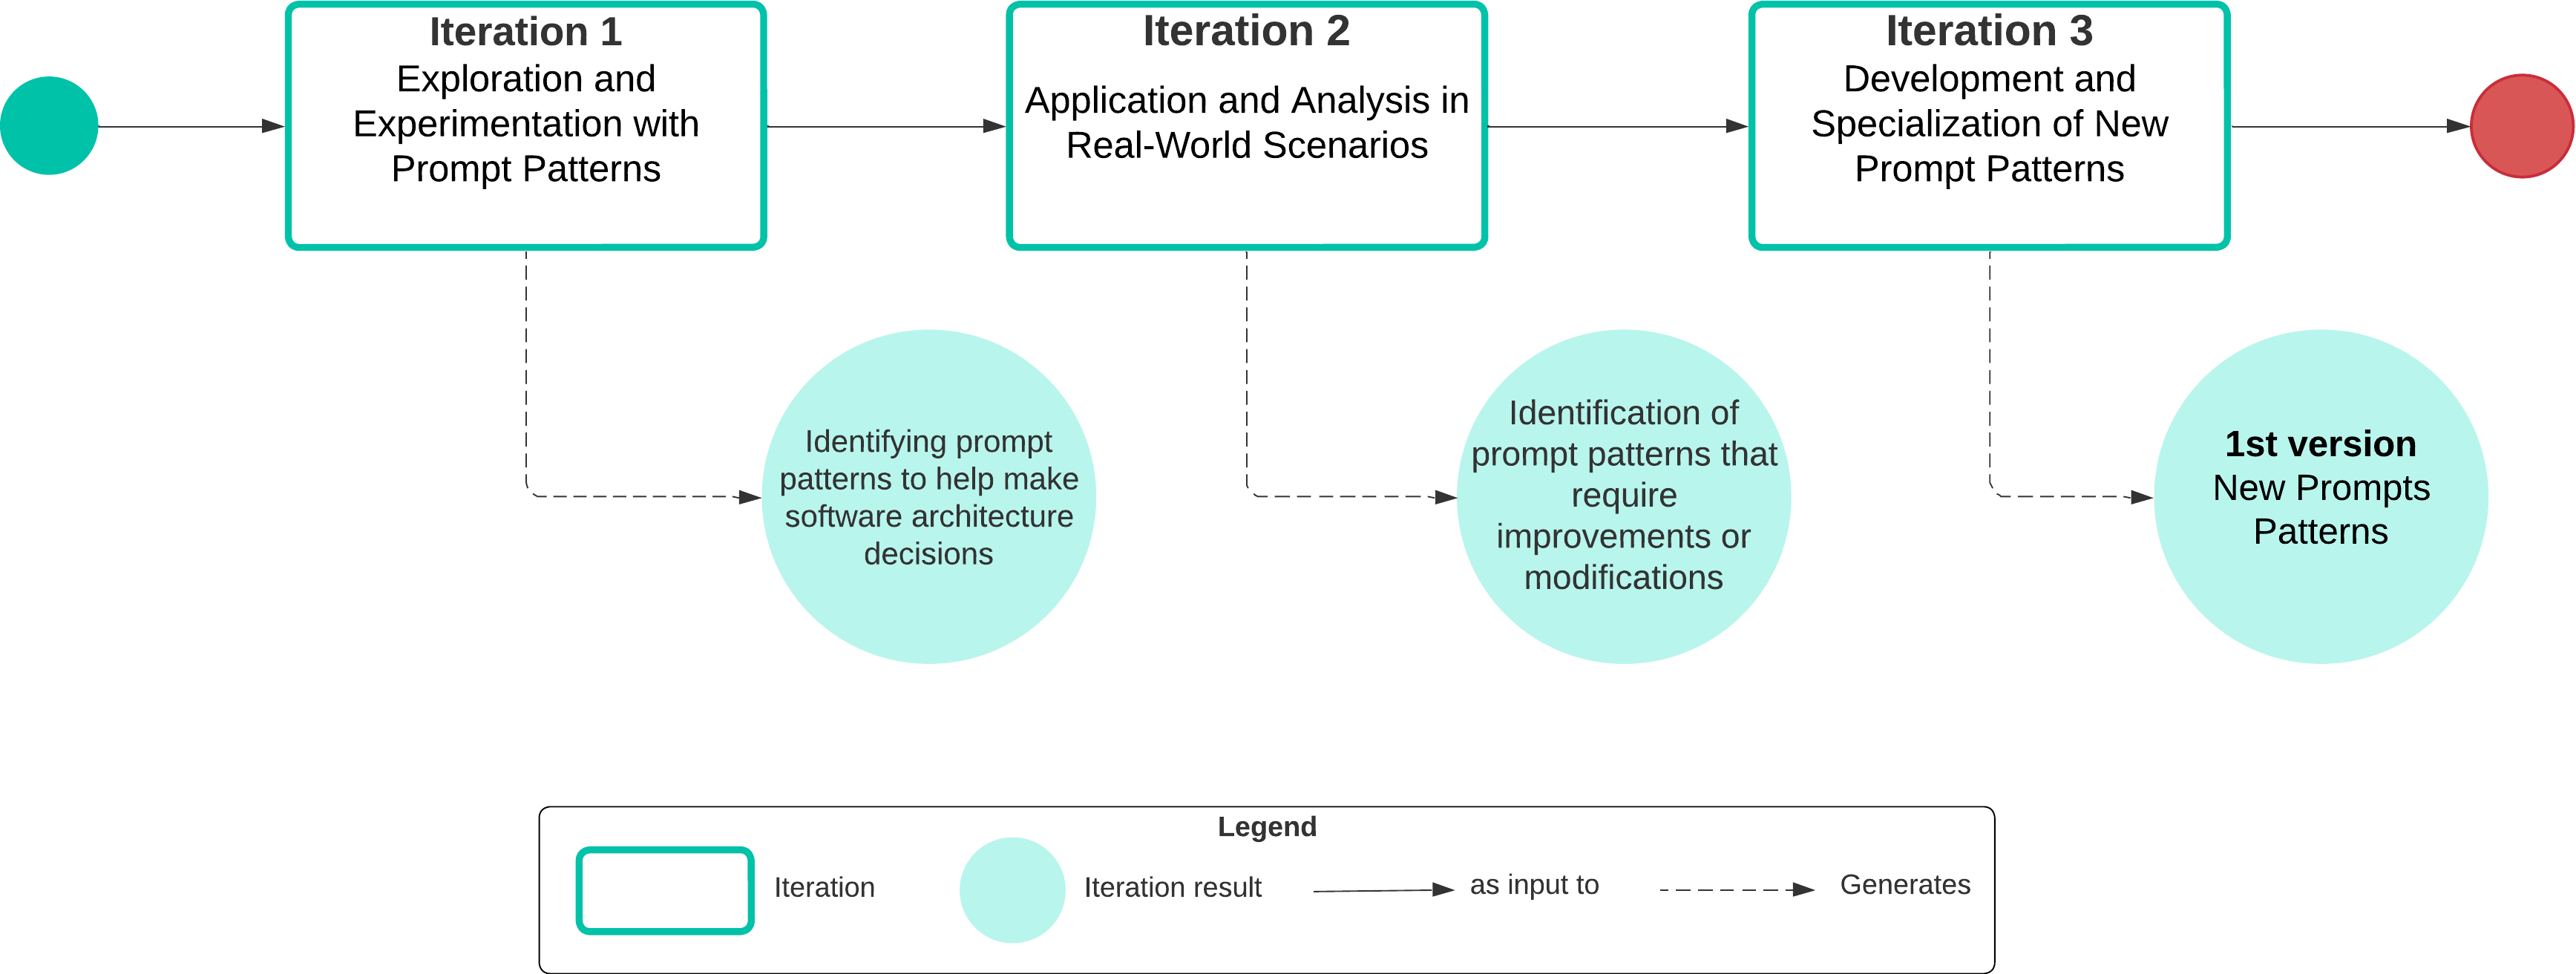
\includegraphics[width=1.0\textwidth]{figures/design-process.png}
\objectsource{\objectsourceauthor}
\end{figure}
% End Figure ---------------------------


\MyParaBold{Iteration 1:} Identifying Prompt Patterns

\begin{itemize}
    \item \textbf{Goal}: The objective is to research and identify relevant prompt patterns to help guide software architecture decision-making.
    \item \textbf{Process:} Conducted a literature review to identify existing prompt patterns. Next, experimented with these patterns using fictitious cases that simulated common problems in software architecture. Finally, the most promising patterns were selected based on their performance in these cases.
    \item \textbf{Result:} Identified several interesting prompt patterns with potential applications in software architecture.
\end{itemize}

\MyParaBold{Iteration 2:} Application and Analysis in Real Contexts
\begin{itemize}
    \item \textbf{Goal:} This iteration aims to apply the prompt patterns selected in Iteration 1 to real-world scenarios. The objective is to identify areas for improvement in the prompt patterns.
    \item \textbf{Process:} Implement the selected prompt patterns in real case studies, analyze the effectiveness of the prompt patterns and note any deficiencies or necessary improvements.            
    \item \textbf{Result:} This iteration aims to identify specific aspects of the prompt patterns requiring improvement to better address real-world architectural challenges.
\end{itemize}

\MyParaBold{Iteration 3:} Development and Specialization of New Prompt Patterns
\begin{itemize}
    \item \textbf{Goal:} Propose an approach of a sequence of new prompt patterns specializing in existing ones for use in software architecture scenarios.
    \item \textbf{Process:} Develop new prompt patterns to address gaps identified in Iteration 2, specialize existing prompts to make them more applicable to the unique requirements of software architecture, and apply new standards in LLMs that specialize in real scenarios for validation.        
    \item \textbf{Result:}  Establish a refined set of new and adapted prompt patterns(\textit{\textbf{1st version}}), demonstrating their effectiveness in practical applications in software architecture.
\end{itemize}

Per the seven guidelines of Design Science Research (DSR), this structured, iterative process ensures the relevance and applicability of the prompt patterns. The methodical rigor of DSR is evident as each phase builds upon the insights and feedback from the previous one, resulting in a set of prompt patterns ready for deployment in the field of software architecture.

\MyParaBold{Proposed Patterns}

\MyParaText{The following five prompt patterns are proposed in this work and proposed pattern sequence:}
\begin{enumerate}
    \item Software Architect Persona, section \ref{sec:software-architect-persona}
    \item Architectural Company Context, section \ref{sec:architectural-company-context}
    \item Quality Attribute Question, section \ref{sec:quality-attribute-question}
    \item Technical Premises, section \ref{sec:technical-premises}
    \item Uncertain Requirement Statement \ref{sec:uncertain-requirement-statement}
    \item Fictional Scenario to Demonstrate the Pattern-based Prompt Sequence \ref{sec:fictional-scenario-prompt-pattern-sequence}
\end{enumerate}

\MyParaBold{Prompt Pattern Forms}

Defining objective rules for the most appropriate form to describe a specific pattern is difficult. The form depends on the pattern of the author's intention and target audience. Therefore, subjectivity and experience play a crucial role. However, some heuristics can help pattern writers decide which form to use \cite{buschmann2007pattern}.

There are many forms available for documenting patterns, including the structured and detailed \textcite{Gamma1994} and  \textcite{buschmann1996pattern} forms, the narrative 'Portland' form by \textcite{cunningham1995checks}, the form used by \textcite{Alexander1977}, and even unusual forms such as the one developed by \textcite{cockburn1997surviving}, which introduces aspects like the 'overdose' effect of a pattern, reminiscent of the medical diagnostic metaphor.

The Coplien approach is a specific way of documenting design patterns in software engineering introduced by \textcite{coplien1995generative}. It is known for its concise and essence-focused approach to pattern documentation. The main elements of the Coplien form are as follows: \textbf{\textit{1.Name}}, \textbf{\textit{ 3.Problem}}, \textbf{\textit{4.Context}}, \textbf{\textit{5.Forces}}, \textbf{\textit{6.Solution}}, \textbf{\textit{7.Rationale}}, and \textbf{\textit{10.Consequences}} (formally known as Resulting Context).

The Pattern Form used in this work includes additional elements that offer a more practical and comprehensive understanding of how the pattern can be applied in the broader context of design patterns. This work follows the Coplien form but with some extra features, including \textbf{\textit{2.Specializations}}, \textbf{\textit{8.Template Statements}}, \textbf{\textit{9.Concrete Statement Example}}, \textbf{\textit{11.Related Patterns}}, and \textbf{\textit{12.Usage Example}}, which will be explained in detail below:

\MyPara{1.Name:} A concise and descriptive name for the pattern quickly communicates its essence.

\MyPara{2.Specializes:} Should detail how the current standard specializes or extends existing standards, showing the relationship between the current standard and others in the same domain. It focuses on refining or modifying established standards to solve specific problems or contexts.

\MyPara{3.Context:} A description of the situations or conditions under which the problem and the solution are applicable. This section provides the background necessary to understand the circumstances in which the pattern is relevant.

\MyPara{4.Problem:} A clear statement of the problem that the pattern addresses. This section defines the issue the pattern aims to solve, often highlighting the specific context where this problem arises.

\MyPara{5.Forces:} Discuss the "forces" in the problem space. These constraints, trade-offs, or tensions must be balanced when applying the pattern. Understanding these forces helps grasp the problem's nuances and the pattern's appropriateness.

\MyPara{6.Solution:} A description of the solution to the problem, as the pattern proposes. This is not a detailed implementation but rather an abstract description of how to resolve the problem or achieve the desired outcome.

\MyPara{7.Rationale:} Explain why the solution works and how it addresses the forces and the problem. This section often includes insights into the underlying principles or theories that make the pattern effective.

\MyPara{8.Statement Template:} Serves as a quick reference or succinct summary of the standard, providing an immediate overview of what the standard is about. It can be a model statement or a structured summary that encapsulates the essence of the patterns in a standardized format.

\MyPara{9.Concrete Statement Example:} is a real-life example of the declaration template that illustrates how it can be applied in practice.

\MyPara{10.Consequences:} A description of the state or situation after the pattern has been applied, including any new problems that might arise or how the context has been altered due to applying the pattern.

\MyPara{11.Related Patterns:} provides information about other patterns closely related to the current one. It shows dependencies or prerequisites and provides a network of patterns that can work well together or be considered together when solving complex problems.

\MyPara{12.Usage example:} Goes beyond the theoretical explanation and provides a practical, real-world scenario where the pattern is applied. This can be particularly useful for readers to understand the applicability and implementation of the standard.

By including these additional elements, you're enriching the pattern description, making it more practical, and providing a more holistic view of how the pattern fits within the broader context of design patterns. This approach can be especially beneficial for practitioners looking to apply these patterns in real-world scenarios.



\section{The Software Architect Persona Pattern} \label{sec:software-architect-persona}

\MyPara{Name:} Software Architect Persona

\MyPara{Specializes:}\texttt{Persona}

\MyPara{Context:} People interacting with LLM often need responses considering their perspective, experience, or context. To make decisions, software architects must balance functional and non-functional requirements, software business rules, and their constraints and goals. A customized persona can be assigned specific roles, specialties, objectives, and limitations to overcome this challenge. By using these resources, communication with LLM can be structured, and responses to the user can be consistent and appropriate to their context.

\MyPara{Problem:} How can we make requests more accurate by incorporating roles, experts, objectives, and limitations into AI-generated content while maintaining coherence with users' perspectives and contexts?

\MyPara{Forces:} The following are forces in using Software Architect Persona:
\newline
- \textit{Scope limitation:} A software architect has limited decision-making power and should not suggest solutions outside their role.
\newline
- \textit{Prompt answer applicability:} An answer that suggests a solution out of the architect's decision power would not be useful.
\newline
- \textit{Simple persona usage:} An architect can have different roles and responsibilities in different contexts, and only declaring their role in the prompt might not be enough.

\MyPara{Solution:} Create a prompt that describes the software architect's role and limitations regarding the target design decision.

\MyPara{Rationale:} The rationale behind the Software Architect Persona pattern is to enhance the relevance and accuracy of AI-generated responses for software architects. The responses become more aligned with the user's context and perspective by embedding specific roles, expertise, objectives, and limitations into the AI interaction.

\MyParaText{This is achieved by creating prompts that clearly outline the software architect's role, goals, and constraints regarding the targeted design decision. This ensures that the AI's responses are technically accurate and contextually appropriate, aiding in more effective decision-making.}


\MyPara{Statement Template:}You are \textcolor{mycolorgreen}{[\textbf{Persona's Name}]} in the role \textcolor{mycolorgreen}{\textbf{[Role]}}.Your main goal is \textcolor{blue}{\textbf{[Main Goal]}.}You cannot \textcolor{mycolorpink}{\textbf{[Limitations/Constraints]}}.

\MyParaBold{\textcolor{mycolorgreen}{-[Persona's Name]:}} This variable represents the specific identity or role of the software architect. It helps to personalize the AI’s response by giving it a clear subject to address.

\MyParaBold{\textcolor{mycolorgreen}{-[Role]:}} This details the specific role or responsibility of the software architect within the context of the project, helping to define the scope and focus of the AI’s responses.

\MyParaBold{\textcolor{blue}{-[Main Goal]:}} This outlines the primary goal or objective that the software architect is aiming to achieve. This guides the AI in generating responses aligned with achieving these specific goals.

\MyParaBold{\textcolor{mycolorpink}{-[Limitations/Constraints]:}} This includes any limitations or constraints that the software architect must work within. Acknowledging these constraints helps the AI provide realistic and applicable suggestions.

\MyPara{Concrete statement example:}\textbf{ \textcolor{mycolorgreen}{You are a Senior Software Architect specializing in cloud-based solutions.}\textcolor{blue}{Your main goal is to optimize system scalability and performance.} \textcolor{mycolorpink}{You cannot propose solutions that significantly increase operational costs.}}

\MyPara{Consequences:} The following are consequences of using Software Architect Persona: 
\newline
\textcolor{red}{(-)} It requires more effort to define the persona in advance and ensure that the instructions are aligned with it \newline
\textcolor{red}{(-)} May limit response flexibility if constraints are too narrow\newline
\textcolor{red}{(-)} Persona can introduce unintentional biases if not well defined\newline
\textcolor{red}{(-)} May produce less natural or creative responses when imposing the persona\newline
\textcolor{blue}{(+)} Get answers specifically adapted to your needs and context\newline
\textcolor{blue}{(+)} Get more realistic and consistent advice by simulating a knowledge expert\newline
\textcolor{blue}{(+)} Avoid unfiltered or off-topic responses\newline
\textcolor{blue}{(+)} Clear guidance on appropriate and expected response types\newline
\textcolor{blue}{(+)} Less ambiguity in prompts, which helps generate more focused responses\newline
\textcolor{blue}{(+)} Greater probability of a more accurate answer, avoiding topics outside the scope

\MyPara{Related Patterns:} This pattern specializes \texttt{Persona} by adding more details on the Persona decision scope and the limitations. This pattern is related to \texttt{Context Manager} because it is also a way to limit the scope of the answer.

\MyPara{Usage example:} Created an example prompt to test the effectiveness of Persona on ChatGPT. The objective is to verify whether the LLM can assign the persona in the software architect's domain. For more information, full prompt at the following link: \href{https://chat.openai.com/share/ee2385fe-0040-4468-9db7-72d8e6bd2864}{Software Architect Persona}.

\begin{chatin}{usercolor}{\chatgptin[chatgpt-in-persona-1]}

From now on, you are Neo in the role of an experienced software architect. Your main goal is to ensure the reliability, performance, and maintainability of the software for which you are responsible. You have experience designing scalable and secure systems. You cannot under any circumstances resolve doubts and questions that involve other topics or subjects that are not Software Architecture, such as code implementation, so respond that it is not your persona's responsibility.
\end{chatin}

In Prompt \ref{chatgpt-in-persona-1}, the persona`s name was defined as a role, a goal, and limitations.

\begin{chatout}{botbubble}{\chatgptout[chatgpt-out-persona-1]}

As "Neo" the software architect, I'm ready to assist you with any questions or challenges related to software architecture, including system design, scalability, reliability, performance, and maintainability. If you have questions in these areas or need advice on architectural patterns and practices, feel free to ask.
\end{chatout}

\begin{chatin}{usercolor}{\chatgptin[chatgpt-in-persona-2]}
Summarize in 2 paragraphs the best strategies or techniques for migrating a monolithic system with MVC architecture to a microservices system?
\end{chatin}


\begin{chatout}{botbubble}{\chatgptout[chatgpt-out-persona-2]}

When migrating a monolithic system with an MVC (Model-View-Controller) architecture to a microservices architecture, the first step is typically to identify and segregate bounded contexts. This involves breaking down the monolith into domains that represent discrete business capabilities. You would assess the model layer for business logic that can be decoupled and organized into independent services. An incremental approach is often recommended, where you start by carving out the least dependent modules and gradually work towards the more complex ones, ensuring that the monolith and new microservices can coexist during the transition phase. This is known as the Strangler Fig Pattern, where new microservices gradually "strangle" the old monolith until it is eventually decommissioned.

In terms of techniques, it's crucial to establish a robust communication mechanism between microservices, which can be achieved through APIs or messaging queues. Interim APIs can serve as a bridge between the monolith and new microservices. It's also important to implement a comprehensive testing strategy to ensure that as each microservice is extracted, the system continues to function as expected. Continuous Integration / Continuous Deployment (CI/CD) pipelines are vital to maintain a smooth and reliable delivery process during the transition. Finally, you need to address cross-cutting concerns such as authentication, logging, and monitoring at the microservices level, often using sidecars or external services. These strategies ensure not only a smooth transition but also the maintainability and scalability of the new microservices architecture.
\end{chatout}

During a conversation in the "Neo" persona, ChatGPT recognized its limitations in non-architectural tasks. However, it provided successful strategies for migrating to a micro-service architecture, as shown in Prompt \ref{chatgpt-in-persona-1}, Output \ref{chatgpt-out-persona-1} and  \ref{chatgpt-out-persona-2}.

\begin{center}
                       
\end{center}

\section{The Architectural Company Context Pattern} \label{sec:architectural-company-context}

\MyPara{Name:} Architectural Company Context

\MyPara{Specializes:} \texttt{Reflection}

\MyPara{Context:} In the dynamic software development environment, architectural decisions are significantly influenced by three critical factors: the maximum development time available for creating or modifying software, the development team size, and the project budget.

\MyPara{Problem:}How can software architects create an architecture that aligns with business and technical requirements while effectively navigating practical constraints of development time, team size, and budget without compromising software quality and functionality?

\MyPara{Forces:} The following are forces in using Architectural Company Context:
\newline
- \textit{Realistic architectural solutions:} enables the creation of viable architectural solutions considering the budget, team size, and development schedule, reducing the risk of delays and project failures.
\newline
- \textit{Alignment with Business Objectives:} Important information so that architectural decisions must be aligned with business objectives to support the company's strategic direction.
\newline
- \textit{Risk Mitigation:} Identifying potential risks early in the architectural design process can avoid costly mistakes and ensure a safer, more compliant architecture.
\newline
- \textit{Helps decision-making:} The pattern improves architectural decision-making, improving project results and satisfaction.


\MyPara{Solution:}Create a prompt that evaluates whether the proposed Architecture is implementable based on development time, team size, and available budget. 

\MyPara{Rationale:} The rationale behind the Architectural Company Context pattern is to ensure that architectural decisions are grounded in the reality of the company's constraints. It emphasizes the alignment of software architecture with the practical limitations and opportunities presented by time, team size, and budget.
 
\MyParaText{This pattern helps architects create architecture that is not only theoretically sound but also practically feasible. Considering these constraints, architects can make informed decisions that balance quality, functionality, and practicality.}

\MyPara{Statement Template:} Given a development timeline of \textcolor{mycolorgreen}{\textbf{[Time]}}, a team of \textcolor{blue}{\textbf{[Team Size]}}, and a budget of \textcolor{mycolorpink}{\textbf{[Budget]}}, determine if the proposed architecture \textcolor{mycolororange}{\textbf{[Architecture Description]}} is feasible and can meet the project requirements without compromising on quality.

\MyParaBold{\textcolor{mycolorgreen}{[Time]:}}This variable represents the maximum development time available for the project. It sets the timeline within which the architecture must be designed and implemented, influencing decisions about complexity and scope. 

\MyParaBold{\textcolor{blue}{[Team Size]:}}This refers to the number of team members involved in the project. It affects the division of labor and the team's complexity level to manage and implement effectively. 

\MyParaBold{\textcolor{mycolorpink}{[Budget]:}}This variable indicates the financial resources allocated for the project. It determines the feasibility of certain architectural choices, especially those involving new technologies or significant investment. 

\MyParaBold{\textcolor{mycolororange}{[Architecture Description]:}}This is a brief description of the proposed architectural approach or style (e.g., microservices, monolithic). It is the subject of evaluation against time constraints, team size, and budget.
       
\MyPara{Concrete Statement Example:}\textbf{\textcolor{mycolorgreen}{Given a development timeline of 6 months, }\textcolor{blue}{a team of 10 developers, }\textcolor{mycolorpink}{and a budget of \$500,000.00, }\textcolor{mycolororange}{determine if implementing a microservices-based architecture for our e-commerce platform is feasible and can deliver the required scalability and performance within these constraints.}
}

\MyPara{Consequences:} 
\newline
\textcolor{red}{(-)} May restrict innovation or the adoption of ideal architectural practices due to practical limitations.\newline
\textcolor{red}{(-)} It might lead to conservative choices, potentially overlooking cutting-edge or innovative architectural solutions.\newline
\textcolor{red}{(-)} It can create a risk-averse culture where teams might shy away from ambitious or experimental approaches due to perceived constraints.\newline
\textcolor{blue}{(+)} Encourages efficient resource management, optimizing time, team capabilities, and budget.\newline
\textcolor{blue}{(+)} Promotes pragmatic decision-making, focusing on what is achievable and sustainable in the given context.\newline
\textcolor{blue}{(+)} Leads to the development of realistic, feasible architectural solutions that are tailored to the company's specific context.

\MyPara{Related Patterns:} The Architectural Company Context is related to the  \texttt{Reflection} pattern as it requires continuous reassessment and adaptation of the architecture to align with changing company contexts, resources, and constraints.

\MyPara{Usage example:} Created an example prompt that uses the Architectural Company Context pattern to assist in making decisions related to software architecture. The prompt involves four variables - Time, Time Size, Budget, and Architectural Description, as shown in Prompt \ref{chatgpt-in-company-1}. This example will help demonstrate how the pattern can be applied in real-world scenarios. You can choose to remove any variables that are not relevant to the context and requirement of the software architect's decision-making process. For more information, full prompt at the following link: \href{https://chat.openai.com/share/5b124d5f-cc5e-422c-ab11-b932d482de1d}{Architectural Company Context}.

\begin{chatin}{usercolor}{\chatgptin[chatgpt-in-company-1]}

Given a 6-month development timeline, a team of 10 developers, and a budget of \$500,000.00, determine whether implementing a microservices-based architecture for a new, non-existent e-commerce platform is feasible and can provide scalability. and performance required within the constraints of time, staff, and budget.
\end{chatin}
    
ChatGPT highlighted some factors that need to be considered, such as qualified developers with experience in microservices and distributed systems. These are crucial to success, especially for e-commerce platforms where complexity can significantly impact the project. The technology stack and tools used significantly impact development speed and costs. Agile methodologies are suitable for microservices, providing flexibility in development. However, hosting microservices is challenging due to the need for robust infrastructure and comprehensive testing strategies. Operating a large-scale microservices architecture often requires additional tools and knowledge to manage many services efficiently.

After analyzing the factors above, ChatGPT responded by listing the variables Timeline, Team, and Budget. As shown in Output \ref{chatgpt-out-company-1}.

\begin{chatout}{botbubble}{\chatgptout[chatgpt-out-company-1]}
\begin{itemize}
    \item \textbf{Timeline:} 6 months is a relatively short time for building a microservices-based e-commerce platform from scratch, especially considering the complexity of both the architecture and the business domain.    
    \item \textbf{Team:} 10 developers could be sufficient if they are experienced in microservices, but it might be tight considering the need for specialized roles (e.g., DevOps, backend/frontend developers, QA engineers).    
    \item \textbf{Budget:} \$500,000 might be adequate for the development phase, but consider additional costs for infrastructure, tools, and post-launch maintenance and support.
\end{itemize}
\end{chatout}
    
\begin{center}
                       
\end{center}

\section{The Quality Attribute Question Pattern} \label{sec:quality-attribute-question}

\MyPara{Name:} Quality Attribute Question

\MyPara{Specializes:}\texttt{Question Refinement}

\MyPara{Context:} Software architecture is crucial in meeting functional and non-functional requirements while maintaining desired quality attributes. This is achieved by selecting appropriate architectural patterns, technologies, and design strategies. The critical challenge is systematically identifying and addressing these attributes, ensuring a balanced and effective architectural design during software construction or maintenance.

\MyPara{Problem:} How can generative AI help architects discover and evaluate quality attributes when making architectural decisions?

\MyPara{Forces:} The following are forces in using Quality Attribute Question:
\newline
- Integration of different quality attributes based on the system’s functional and non-functional requirements.
\newline
- Clarification of the feasibility of implementing requested functional and non-functional requirements, balancing these with technical difficulties and project conditions.
\newline
- Reduction of unpredictability by identifying quality attributes that might otherwise be overlooked.
\newline
- Personalization of responses to fit the specific context of the architectural question.

\MyPara{Solution:} Create a prompt pattern that leverages the synthetic knowledge of generative AI to extract and evaluate quality attributes in an approach where the AI can analyze and ask about the software context to collect information for later architectural decision-making.

\MyPara{Rationale:} The logic behind the Quality Attribute Question Pattern is to help with architectural decision-making through quality attributes so that generative AI can ask the architect questions about the software context to give more precise guidance on the architectural decision.
 

\MyPara{Statement Template:} You are \textcolor{mycolorgreen}{\textbf{[Role]}} responsible for \textcolor{blue}{\textbf{[Description Project]}}. Your primary focus is to design an architecture that excels in \textcolor{mycolorpink}{\textbf{[List Of The Quality Attribute]}}. Your task is  \textcolor{mycolororange}{\textbf{[Decision-making Process]}}. You should ask  \textcolor{mycolorlilas}{\textbf{[Clarify Doubts]}}. \textcolor{mycolorblue}{\textbf{[Recommendations]}}. Additionally, provide a \textcolor{mycolorred}{\textbf{[Comprehensive Prompt].}}

\MyParaBold{\textcolor{mycolorgreen}{[Role]:}} Define the role and responsibilities of the software architect.

\MyParaBold{\textcolor{blue}{[Description Project]:}} Explain the project requirements, essential considerations, and client/user preferences.

\MyParaBold{\textcolor{mycolorpink}{[List Of The Quality Attribute]:}} Specify the expectations for each quality attribute.

\MyParaBold{\textcolor{mycolororange}{[Decision-making Process]:}} Describe the decision-making process, priorities, and system structure.

\MyParaBold{\textcolor{mycolorlilas}{[Clarifying Doubts]:}} Please ask the Software Architect if there are any questions.

\MyParaBold{\textcolor{mycolorblue}{[Recommendations]:}} Provide recommendations or advice for the generative AI.

\MyParaBold{\textcolor{mycolorred}{[Comprehensive Prompt]:}} Provide a prompt that includes the outcome of architectural decision-making information and the rationale for the choices.

\MyPara{Concrete Statement Example:} \textbf{\textcolor{mycolorgreen}{You are an experienced software architect responsible for}  \textcolor{blue}{creating a credit card processing system for a medium-sized financial institution.} \textcolor{mycolorpink}{Your primary focus is to design an architecture that excels in scalability, security, and performance.} \textcolor{mycolororange}{Your task is to carefully navigate through the decision-making process of the credit card processing system architecture, step by step.}  \textcolor{mycolorlilas}{You should ask any necessary questions to clarify doubts about the quality attributes of the new system.} \textcolor{mycolorblue}{Avoid making any architectural decisions until all questions are answered.} \textcolor{mycolorred}{Additionally, provide a comprehensive prompt that includes all the data collected in the previous steps, along with an explanation of the rationale behind each architectural decision-making.}}

\MyPara{Consequences:}
\newline
\textcolor{blue}{(+)} Promotes a deeper understanding of each quality attribute, leading to well-informed architectural decisions. \newline
\textcolor{blue}{(+)} Enhanced Architectural Robustness: Leads to more resilient and adaptable architecture. \newline
\textcolor{blue}{(+)} Increased Stakeholder Confidence: Builds trust and assurance among project stakeholders. \newline
\textcolor{blue}{(+)} Improved Risk Management: Early identification and mitigation of potential issues. \newline
\textcolor{blue}{(+)} Better Alignment with Business Goals: Ensures the architecture effectively meets business and user needs. \newline
\textcolor{blue}{(+)} Enhanced Documentation Quality: Results in more detailed and informative architectural documentation. \newline
\textcolor{red}{(-)} Potentially prolong the decision-making process due to the extensive nature of the questioning. \newline
\textcolor{red}{(-)} Extended Planning Phase: Prolongs the initial planning and decision-making process. \newline
\textcolor{red}{(-)} Possible Delays in Decision-Making: Slows down the overall progress, especially in time-sensitive projects. \newline
\textcolor{red}{(-)} Increased Need for Expertise: Requires a high level of knowledge and experience to implement effectively. \newline
\textcolor{red}{(-)} Risk of Scope Creep: Focusing on multiple attributes might lead to expanding the project beyond its original scope. \newline


\MyPara{Related Patterns:} This pattern is closely linked to Question Refinement. In software architecture, this refers to sharpening and focusing questions to extract more precise and valuable information. The Quality Attribute Question Pattern refines this approach by systematically tailoring questions to address each relevant quality attribute of the software, ensuring a comprehensive evaluation that leads to informed architectural decisions.


\MyPara{Usage example:} Used ChatGPT and created an example prompt that uses the Quality Attribute Questions pattern to validate the interaction with generative AI to help make decisions related to the software's quality attributes. The prompt involves the same variables described in the State Template part and the same prompt as the Concrete Statement Template. The Prompt \ref{chatgpt-in-quality-attribute-question-1} shows the pattern is applied in ChatGPT.For more information, full prompt at the following link: \href{https://chat.openai.com/share/82a67e08-53b6-4b53-b69e-7881954721f2}{Quality Attribute Question}.

\MyParaBold{Iteration 1:} Running Quality Attribute Question

\begin{chatin}{usercolor}{\chatgptin[chatgpt-in-quality-attribute-question-1]}

You are an experienced software architect responsible for creating a credit card processing system for a medium-sized financial institution. Your primary focus is to design an architecture that excels in scalability, security, and performance. 

Your task is to carefully navigate through the decision-making process of the credit card processing system architecture, step by step. You should ask any necessary questions to clarify doubts about the quality attributes of the new system. Avoid making any architectural decisions until all questions are answered. 

Additionally, provide a comprehensive prompt that includes all the data collected in the previous steps, along with an explanation of the rationale behind each architectural decision-making.
\end{chatin}

After running the Prompt \ref{chatgpt-in-quality-attribute-question-1} Quality Attribute Questions Prompt Pattern, ChatGPT reported that designing a credit card processing system for a mid-sized financial institution is a complex task that requires careful consideration of several vital factors. 

To ensure that the architecture excels in scalability, security, and performance, several issues need to be addressed, and several questions need to be asked.

\MyParaBold{Iteration 2:} Questions requested by ChatGPT 
\begin{table}[ht]
    \centering
    \footnotesize    
    \setlength{\tabcolsep}{10pt}
    \board{Questions requested by ChatGPT and our answers }
    \label{board:quality-attribute-questions}
    \begin{tabularx}{\textwidth}{|c|X|X|}  \hline    
        \rowcolor{gray!19} \textbf{Nº} & \textbf{Questions ChatGPT} & \textbf{ Our Answers} \\ \hline
        1 & What is the current transaction volume and what growth do you foresee for the next 5 years? & 100 thousand transactions per day. \\
        \rowcolor{gray!19}
        2 & Are there any specific scalability concerns, such as peak times with exceptionally high transaction volumes? & Yes, peak times and shopping seasons such as Christmas, Children's Day and Black Friday. \\        
        3 & What are the compliance requirements that the system must comply with? & Must comply with PCI DSS and LGPD. \\
        \rowcolor{gray!19}
        4 & Are there specific data security measures that you want to implement? & Encryption and tokenization. \\        
        5 & How should the system handle security updates and vulnerability management? & Security updates must be made according to the degree of vulnerability of the system, the more critical the faster the action must be. \\
        \rowcolor{gray!19}
        6 & What are the expected response times for processing transactions? & Maximum 10 seconds per transaction. \\        
        7 & Are there high availability or disaster recovery requirements? & The system must be recovered within a maximum of 30 minutes after the disaster. \\
        \rowcolor{gray!19}
        8 & Are there existing systems or infrastructures with which the new system needs to integrate? & BACEN and other credit operators. \\        
        9 & What are the preferred technologies or platforms (if any)? & High performance and easy development technologies. \\
        \rowcolor{gray!19}
        10 & What is the budget for both initial development and ongoing maintenance? & 20 million dollars. \\        
        11 & Do you have preferences between cloud-based solutions and on-premises solutions? & Indifferent \\
        \rowcolor{gray!19}
        12 & Who are the main users of the system? & E-commerce and point of sale \\        
        13 & Are there specific legal or regulatory considerations in the regions where the system will be used? & Initially Brazilian financial system \\
        \rowcolor{gray!19}
        14 & What are the expectations for system maintenance and support? & 24 by 7 \\        
        15 & Are there any anticipated future developments for which the system should be prepared (e.g. new technologies, changes in market trends)? & Initially not, but the system should be designed for constant change \\
        \hline
    \end{tabularx}
    \objectsource{\objectsourceauthor}
\end{table}
  

\MyParaBold{Iteration 3:} Summary of ChatGPT's response
The proposed digital transaction system is designed for high scalability, capable of handling double the current transaction volume, especially during peak times like Christmas, Children's Day, and Black Friday. It prioritizes security, adhering to PCI DSS and LGPD standards, and employs encryption and tokenization for data protection. Performance is optimized to ensure transaction response times within 10 seconds, supported by a redundant architecture for high availability and disaster recovery.

The system will seamlessly integrate with BACEN and other credit operators, focusing on high-performance, easy-to-develop technologies. It has a budget of \$20 million for development and maintenance, with a recommendation for a cloud-based solution. User-friendly interfaces are designed for both e-commerce and point-of-sale transactions, along with a customizable administrative dashboard.

Compliance with Brazilian financial regulations is a key legal consideration. The system offers robust 24/7 support and maintenance, with a dedicated team for updates and troubleshooting. Future-proofing is addressed through a modular and flexible architecture, allowing for easy updates and scalability to adapt to technological advancements and market changes.

To create a secure credit card processing system that aligns with your financial institution's objectives and requirements, ChatGPT designed the architectural framework outlined below and presented in Output \ref{chatgpt-out-quality-attribute-question-2}, which is robust and scalable.

\begin{chatout}{botbubble}{\chatgptout[chatgpt-out-quality-attribute-question-2]}
\begin{enumerate}
    \item \textbf{Microservices Architecture: }To ensure scalability and ease of maintenance.
    \item \textbf{Cloud Infrastructure:} For scalability and cost-effectiveness.
    \item \textbf{API Gateway:} To manage and secure interactions between different services.
    \item \textbf{Data Encryption and Tokenization:} For security and compliance.
    \item \textbf{Load Balancers and Auto-Scaling:} To handle peak loads efficiently.
    \item \textbf{Distributed Database System:} For performance and high availability.
    \item \textbf{Continuous Integration/Continuous Deployment (CI/CD):} For rapid and reliable software delivery.
    \item \textbf{Monitoring and Logging:} For real-time monitoring and troubleshooting.
\end{enumerate}
This architecture aims to create a robust, scalable, and secure credit card processing system, aligning with your financial institution's objectives and requirements.
\end{chatout}

\begin{center}
                       
\end{center}

\section{The Technical Premises Pattern} \label{sec:technical-premises}

\MyPara{Name:} Technical Premises

\MyPara{Specializes:}\texttt{Fact Check List}

\MyPara{Context:} The use of generative AI can lead to issues of hallucinations, which LLMs can sometimes address.In the complex software architecture world, validating information provided by Large Language Models (LLMs) is crucial. Ensuring the accuracy and reliability of the data used in architectural decisions is essential for the success of any project.

\MyPara{Problem:} How can a Software Architect validate the technical premises provided by LLMs to ensure that the information used in necessary architectural decisions is accurate and reliable?

\MyPara{Forces:} The following are forces in using Technical Premises:
\newline
- The necessity for accurate and dependable information in making architectural decisions.
\newline
- The challenge in deciphering the rationale behind the LLM's responses.
\newline
- Ensure that LLM results are aligned with the project's technical requirements and constraints.
    
\MyPara{Solution:} The Technical Premises Pattern was designed to guide Software Architects in validating information provided by LLMs. This involves the LLM explaining the logic behind each statement and providing a list of technical premises considered in its answers. This process helps architects critically evaluate LLM results and ensure they are aligned with the technical realities of the project.

\MyPara{Rationale:} This pattern is designed to bridge the gap between AI-generated suggestions and practical architectural requirements, enabling architects to make informed decisions based on verified information.

\MyPara{Statement Template:} \textbf{\textcolor{mycolorgreen}{[Context]}} and \textbf{\textcolor{blue}{[List of Technical Premises]}}.From now on, make sure that when generating a response, the AI language model creates a set of specific facts for each technical premise and justification for each architectural decision-making. These facts should be verified and listed at the end of the output.

\MyParaBold{\textcolor{mycolorgreen}{[Context]:}} Insert the specific context of the project.

\MyParaBold{\textcolor{blue}{[List of Technical Premises]:}} [List out the key technical premises provided by the LLM.

\MyPara{Concrete Statement Example:}\textbf{\textcolor{mycolorgreen}{Project: Development of a Smart Home Automation System. Objective: Design a comprehensive system that integrates various home automation devices (like thermostats, lighting, security cameras, and smart appliances) to provide a seamless, efficient, and user-friendly experience for homeowners.} \textcolor{blue}{List of Technical Premises: Interoperability, User Privacy, Energy Efficiency, User Interface Design, and Scalability.}}\textbf{From now on, make sure that when generating a response, the AI language model creates a set of specific facts for each technical premise and justification for each architectural decision-making. These facts should be verified and listed at the end of the output(Facts, Rational, Architectural Decision-making) informative but succinct in a dissertation format.}

\MyPara{Consequences:}
\newline
\textcolor{blue}{(+)} \textit{Improved Accuracy of Architectural Decisions:} By validating the technical premises of LLM outputs, architects can ensure that the decisions are based on accurate and reliable information. \newline
\textcolor{blue}{(+)} \textit{Increased Understanding of LLM Rationale:} This pattern provides insights into the LLM's thought process, helping architects understand why certain recommendations were made. \newline
\textcolor{blue}{(+)} \textit{Enhanced Trust in LLM Outputs:} Through thorough validation, architects can build greater trust in the reliability and relevance of the LLM's suggestions. \newline
\textcolor{blue}{(+)} \textit{Better Alignment with Project Goals:} By scrutinizing the LLM's reasoning, architects can ensure that the proposed solutions align more closely with the project's specific technical requirements and constraints. \newline
\textcolor{red}{(-)} \textit{Potential Delay in Decision-Making:} The process of validating each technical premise can be time-consuming, potentially slowing down the overall architectural planning and decision-making process. \newline
\textcolor{red}{(-)} \textit{Increased Cognitive Load on Architects:} Architects may face an additional cognitive burden in critically analyzing and validating the LLM's technical premises.\newline
\textcolor{red}{(-)} \textit{Possibility of Over-Reliance on LLM Justifications:} There is a risk of architects becoming too reliant on the LLM’s explanations, which might not always cover all aspects of a complex architectural scenario. \newline
\textcolor{red}{(-)} \textit{Challenges in Interpreting Complex Explanations:} In some cases, the explanations provided by the LLM might be too technical or complex, making it difficult for architects to derive clear insights. \newline

\MyPara{Related Patterns:}  The \texttt{Technical Premises} complements and enhances the \texttt{Quality Attribute Question} by providing a method for validating the technical premises behind each quality attribute question. While the \texttt{Quality Attribute Question} focuses on systematically querying each relevant quality attribute to ensure their thorough assessment, the \texttt{Technical Premises} aids in substantiating the responses and premises made by Large Language Models (LLMs) regarding these attributes. This relationship ensures that the architectural decisions are not only based on a comprehensive evaluation of quality attributes but also on validated and reliable information. Therefore, using these patterns in conjunction enables architects to make more informed and accurate decisions by combining a deep understanding of quality attributes with a critical evaluation of the technical underpinnings provided by LLMs.

\MyPara{Usage Example:} Used ChatGPT and created an example prompt that uses the Technical Premises Pattern to validate the interaction with generative AI to help make decisions. The prompt involves the same variables described in the State Template part and the same prompt as the Concrete Statement Template. Prompt \ref{chatgpt-in-premises-1} shows the pattern applied in ChatGPT. For more information, full prompt at the following link: \href{https://chat.openai.com/share/b0a0651d-2e1f-4be3-9995-1d4babdd1da4}{Technical Premises}.

\begin{chatin}{usercolor}{\chatgptin[chatgpt-in-premises-1]}
\noindent
\textbf{Project:} Development of a Smart Home Automation System

\noindent
\textbf{Objective:} Design a comprehensive system that integrates various home automation devices (like thermostats, lighting, security cameras, and smart appliances) to provide a seamless, efficient, and user-friendly experience for homeowners.

\noindent \textbf{List of Technical Premises:}
\begin{enumerate}
    \item \textbf{Interoperability:}  IoT platform supporting diverse communication protocols (like Zigbee, Wi-Fi, and Bluetooth) to ensure interoperability among smart home devices.    
    \item \textbf{User Privacy:}  Recommends implementing end-to-end encryption and regular data audits to enhance user privacy and data security in the smart home system.    
    \item \textbf{Energy Efficiency:}  integration of AI-driven algorithms to optimize energy usage across various devices, potentially reducing overall energy consumption in the smart home.    
\end{enumerate}
From now on, make sure that when generating a response, the AI language model creates a set of specific facts for each technical premise and justification for each architectural decision-making. These facts must be verified and written in a condensed and succinct manner, so as to take up less screen space, at the end of the result as: (Facts, Rationale, Architectural decision making).
\end{chatin}

The proposed smart home automation system is designed with a focus on three fundamental architectural pillars: interoperability, user privacy, and energy efficiency, each addressing crucial aspects of a modern smart home environment.

The architecture of the smart home automation system is strategically developed
around these core principles. Each decision is taken with an eye towards creating a
seamless, secure, and sustainable smart home experience. By melding these technological considerations, the system is poised to deliver an intuitive, efficient, and user-friendly environment for homeowners.

\begin{chatout}{botbubble}{\chatgptout[chatgpt-out-premises-1]}

For the development of a Smart Home Automation System with the given objectives and technical premises, here's a set of specific facts and justifications for each architectural decision-making:

\noindent
\textbf{Technical Premise 1: Interoperability}

\begin{itemize}
    \item \textbf{Facts:} Utilizing a variety of communication protocols (Zigbee, Wi-Fi, Bluetooth) is crucial for connecting a wide range of smart devices, ensuring compatibility and seamless communication.
    \item \textbf{Rationale: }Different devices prefer different protocols for various reasons (range, power consumption, bandwidth). A multi-protocol approach caters to these diverse needs.
    \item \textbf{Architectural Decision Making:} Implement a central IoT platform that supports these protocols. This could involve using multi-protocol gateways or software that can interface with all these standards.    
\end{itemize}
\noindent
\textbf{Technical Premise 2: User Privacy}
\begin{itemize}
    \item \textbf{Facts:} Implementing end-to-end encryption protects data transmission. Regular data audits help in identifying and mitigating privacy risks.
    \item \textbf{Rationale:} In a smart home environment, sensitive personal data is often transmitted. Encryption ensures that this data remains confidential, while audits maintain ongoing security.
    \item \textbf{Architectural Decision Making:} Include robust encryption mechanisms in the system's design and establish a protocol for frequent security and privacy audits.
\end{itemize}

\noindent
\textbf{Technical Premise 3: Energy Efficiency}
\begin{itemize}
    \item \textbf{Facts:} AI-driven algorithms can analyze usage patterns and optimize energy consumption, potentially leading to significant savings.
    \item \textbf{Rationale:} Smart homes often consume substantial energy. AI can automate the process of energy saving by learning user habits and adjusting device operation accordingly.
    \item \textbf{Architectural Decision Making:} Integrate AI-based energy management software that interfaces with all smart devices and can autonomously control them to enhance energy efficiency.    
\end{itemize}
\end{chatout}

According to recommendations given by ChatGPT, see Output \ref{chatgpt-out-premises-1}, the system must support several communication protocols, such as Zigbee, Wi-Fi, and Bluetooth. This ensures smooth device interaction without compatibility issues, creating a simplified smart home ecosystem.
Prioritize end-to-end encryption and routine data audits to protect user data from breaches and hacking attempts, ensuring data remains secure and private.

Use advanced AI algorithms to optimize energy consumption in smart homes. By analyzing usage patterns and environmental data, devices such as thermostats and lighting systems are dynamically adjusted for maximum efficiency. This decision to incorporate AI into energy management provides numerous benefits, including environmental conservation and cost-effectiveness. The goal is to reduce the overall energy footprint of the smart home significantly.

\begin{center}
                       
\end{center}

\section{The Uncertain Requirement Statement Pattern} \label{sec:uncertain-requirement-statement}

\MyPara{Name:} Uncertain Requirement Statement

\MyPara{Specializes:}\texttt{None}

\MyPara{Context:} Uncertainties in software project requirements can significantly impact software architecture and lead to risks later on, especially in rapidly changing technology landscapes and emerging market trends. To mitigate these consequences, software architects should make predictions about implementing requirements that were not initially planned or are uncertain. This would help them make better decisions and adapt the architecture to meet business requirements. By planning for the risks and impacts of not meeting these requirements, software architects can ensure that the software architecture is better aligned with the business needs.

\MyPara{Problem:} How can a software architect effectively manage uncertain or undefined requirements while minimizing the impact on the software architecture and project?

\MyPara{Forces:} The following are forces in using Uncertain Requirement Statement: 
\newline
- Reducing risks associated with uncertain project requirements.
\newline
- Developing a flexible architecture that can adapt to changes
\newline
- Understanding and balancing the potential risks, integrating new technologies or concepts, and balancing innovation with feasibility.

\MyPara{Solution:} The Uncertain Requirements Statement Pattern is a guide that helps software architects identify and deal with uncertain project requirements. This pattern involves informing the software architect about any potential possibilities or information related to the requirements they might have missed. It emphasizes recognizing these uncertainties and considering their potential impact and risks on future changes. This proactive approach helps mitigate the effects of the system architecture's evolution.

\MyPara{Rationale:} This pattern helps manage uncertainty in a structured way, reducing risks, enabling informed decision-making, and fostering proactive adaptation to changes, ensuring the long-term sustainability and relevance of the project.

\MyPara{Statement Template:}  In \textbf{\textcolor{mycolorgreen}{[Project Context]}}, and \textbf{\textcolor{blue}{[Uncertain Aspect]}}.Examine the potential repercussions of not adequately addressing these uncertainties in the system architecture. This assessment will inform our strategic planning and decision-making in software architecture for mitigation, emphasizing the creation of a system that is not only technologically advanced, but also flexible and responsive to regulatory and technological changes.

\MyParaBold{\textcolor{mycolorgreen}{[Project Context:]}} This defines the environment or the specific conditions under which the project is being executed. It includes the nature of the project, its goals, the stakeholder landscape, the market it operates in, and any other relevant environmental factors.

\MyParaBold{\textcolor{blue}{[Uncertain Aspect:]}} This refers to the specific element or feature of the project that is uncertain. It could be a technology, a requirement, a stakeholder need, a regulatory environment, or any other aspect that is not clearly defined or is subject to change. The identification of this uncertain aspect is crucial as it sets the focus for the management of uncertainty.

\MyPara{Concrete Statement Example:} \textbf{\textcolor{mycolorgreen}{When developing a smart city traffic management system,} \textcolor{blue}{the project team faces uncertainties related to evolving regulatory compliance standards and the integration of emerging autonomous vehicle technologies.}  Examine the potential repercussions of not adequately addressing these uncertain requirements in the system architecture. This assessment will inform our strategic planning and decision-making in software architecture for mitigation, emphasizing the creation of a system that is not only technologically advanced, but also flexible and responsive to regulatory and technological changes.}

\MyPara{Consequences:}\newline
\textcolor{blue}{(+)} \textbf{Enhanced Adaptability:} Allows for more flexible and resilient architectural designs that can accommodate changes in requirements or circumstances. \newline
\textcolor{blue}{(+)} \textbf{Improved Risk Management:} By anticipating uncertainties, architects can devise strategies to mitigate potential risks, reducing the likelihood of project setbacks. \newline
\textcolor{blue}{(+)} \textbf{Informed Decision-Making:} Architects gain a deeper understanding of the potential impacts of uncertainties, leading to more informed and strategic choices. \newline
\textcolor{blue}{(+)}\textbf{Proactive Planning:} Encourages forward-thinking and proactive planning, helping to avoid last-minute changes and disruptions. \newline
\textcolor{blue}{(+)} \textbf{Better Stakeholder Alignment: }Clear documentation and communication of uncertainties can lead to more realistic expectations among stakeholders, improving alignment and satisfaction. \newline
\textcolor{red}{(-)} \textbf{Potential for Over-Planning:} Focusing extensively on uncertainties can lead to over-preparation for scenarios that may never materialize, potentially wasting time and resources. \newline
\textcolor{red}{(-)} \textbf{Decision Paralysis:} An overemphasis on every possible uncertainty can lead to indecision or delay in decision-making, hindering project progress. \newline
\textcolor{red}{(-)} \textbf{Increased Complexity:} Managing a wide range of potential scenarios and their implications can add complexity to the architectural planning process. \newline
\textcolor{red}{(-)} \textbf{Resource Allocation Challenges:} Allocating resources effectively becomes more challenging, as it may be unclear where to focus efforts and investment in the face of uncertainties. \newline
\textcolor{red}{(-)} \textbf{Possible Caution Over Innovation:} A strong focus on mitigating risks might lead to overly conservative decisions, potentially stifling innovation and creative solutions. \newline

\MyPara{Related Patterns:}The Uncertain Requirement Statement interacts significantly with two other prominent patterns: \texttt{Fact Check List} and \texttt{Quality Attribute Question}.

The interplay between the \texttt{Uncertain Requirement Statement} and the \texttt{Fact Check List} is primarily complementary. While the \texttt{Fact Check List} is instrumental in confirming verifiable facts and concrete data, the \texttt{Uncertain Requirement Statement} addresses the ambiguities and uncertainties in project requirements. This combination ensures a holistic approach to requirements analysis, balancing the certainty of verified facts with the flexibility to adapt to evolving or unclear project needs.

Similarly, the relationship with the \texttt{Quality Attribute Question} is synergistic. The \texttt{Quality Attribute Question} examines the impact of specific quality attributes on a project. However, uncertain requirements can often obscure the clarity needed in assessing these attributes. The \texttt{Uncertain Requirement Statement} assists here by providing a method to manage and explore these uncertainties, allowing for a more informed and comprehensive evaluation of quality attributes in the context of variable project requirements.

Together, these patterns form a robust framework for decision-making in software architecture, ensuring that a project's known and unknown elements are adequately addressed.

\MyPara{Usage Example:} Used ChatGPT and created an example prompt that uses the Uncertain Requirement Statement Pattern to validate the interaction with generative AI to help make decisions. The prompt involves the same variables described in the State Template part and the same prompt as the Concrete Statement Template. Prompt~\ref{chatgpt-in-uncertain-requirement-1} shows the pattern applied.For more information, full prompt at the following link: \href{https://chat.openai.com/share/4155325e-0d73-4e69-816a-b38df4588660}{Uncertain Requirement Statement}.

\begin{chatin}{usercolor}{\chatgptin[chatgpt-in-uncertain-requirement-1]}

When developing a smart city traffic management system, the project team faces uncertainties related to evolving regulatory compliance standards and the integration of emerging autonomous vehicle technologies. Examine the potential repercussions of not adequately addressing these uncertain requirements in the system architecture. This assessment will inform our strategic planning and decision-making in software architecture for mitigation, emphasizing the creation of a system that is not only technologically advanced, but also flexible and responsive to regulatory and technological changes. Output format, Problem, Impact of not adopting the requirement and architectural decision making.
\end{chatin}


The Output~\ref{chatgpt-out-uncertain-requirement-1} highlights the need for a system architecture that can adapt to changes in regulatory standards. The impact of not doing so includes legal issues, downtime, and expensive modifications. The solution is to implement a modular architecture that allows for easy updates and integration of new compliance modules. 

The ChatGPT addresses the challenge of integrating new autonomous vehicle technologies. System incompatibilities, security concerns, and obsolescence may exist without effective integration. The architectural response involves designing the system with open standards and interfaces and a data management system that can handle diverse and growing data volumes.

The strategy involves developing a flexible and scalable architecture using cloud solutions, microservices, and APIs. Continuously monitoring regulatory and technological trends and feedback loops in the development process ensures adaptability. As shown in Output~\ref{chatgpt-out-uncertain-requirement-1}, collaboration with interested parties keeps the architecture aligned with future changes and requirements.
 
Concentrating on strategic planning elements such as managing risks for regulatory changes and technological advances, investing in research and development for innovative solutions, training the development team in new technologies and standards, and employing agile methodologies for flexibility and rapid adaptation. These measures aim to make the traffic management system resilient, adaptable, and future-proof, especially in the context of smart city infrastructure.

\begin{chatout}{botbubble}{\chatgptout[chatgpt-out-uncertain-requirement-1]}

\noindent
\textbf{Problem: Evolving Regulatory Compliance Standards}

\noindent
\textbf{Impact: }If the system architecture doesn't account for evolving regulations, it might become non-compliant with new laws, leading to legal penalties, system downtime, and costly modifications.

\noindent
\textbf{Architectural Decision-Making:} Implement a modular architecture that allows easy updates and adaptations to new regulations. This approach should include the ability to quickly integrate new compliance modules or update existing ones without disrupting the overall system.

\noindent
\textbf{Problem: Integration of Emerging Autonomous Vehicle Technologies}

\noindent
\textbf{Impact: }Failure to effectively integrate these technologies can result in system incompatibilities, safety issues, and reduced efficiency. The system might become obsolete quickly as newer technologies emerge.

\noindent
\textbf{Architectural Decision-Making:} Design the system with open standards and interfaces to easily incorporate new autonomous vehicle technologies. This should include scalable and flexible data management systems capable of handling increasing volumes and varieties of data from various vehicle technologies.

\noindent
\textbf{General Architectural Strategy for Mitigation}

\noindent
\textbf{Adaptive and Scalable Architecture:} Develop an architecture that is inherently flexible, allowing for scalability and adaptability to technological advancements and regulatory changes. This could involve using cloud-based solutions, microservices, and APIs that support integration and scalability.

\noindent        
\textbf{Continuous Monitoring and Feedback Loops:} Establish mechanisms for ongoing monitoring of regulatory and technological trends. Implement feedback loops in the development process to ensure the architecture can adapt and evolve as required.

\noindent
\textbf{Stakeholder Collaboration:} Engage with regulators, technology providers, and other stakeholders to stay informed about upcoming changes and requirements. This collaboration can inform the architectural design, ensuring it meets current and anticipated needs.

\noindent
\textbf{Strategic Planning Considerations:} Develop a risk management plan focusing on potential regulatory changes and technological advancements. Regularly review and update this plan.

\end{chatout}

\begin{center}
                       
\end{center}

\section{Fictional Scenario to Demonstrate the Prompt Patterns Sequence} \label{sec:fictional-scenario-prompt-pattern-sequence}

In sections \ref{sec:software-architect-persona}, \ref{sec:architectural-company-context}, \ref{sec:quality-attribute-question}, \ref{sec:technical-premises}, and \ref{sec:uncertain-requirement-statement} of our work, introduces five different prompt patterns to help users gain insights into their software architecture. These patterns are as follows: \texttt{Software Architect Persona}, \texttt{Architectural Company Context}, \texttt{Quality Attribute Question}, \texttt{Technical Premises}, and \texttt{Uncertain Requirement Statement} respectively. Each pattern can be used independently or combined, allowing bypassing, as illustrated in the Prompt Pattern Sequence Decision Flow in Figure~\ref{flowchart-pattern}. 

However, combining them in a specific sequence can yield more valuable insights. To test this hypothesis, we conducted experiments with software architects in companies and identified an ideal sequence of prompts.

\begin{figure}[!ht]
    \centering
    \caption{\centering Decision Flow To Prompt Patterns Sequence}\label{flowchart-pattern}
    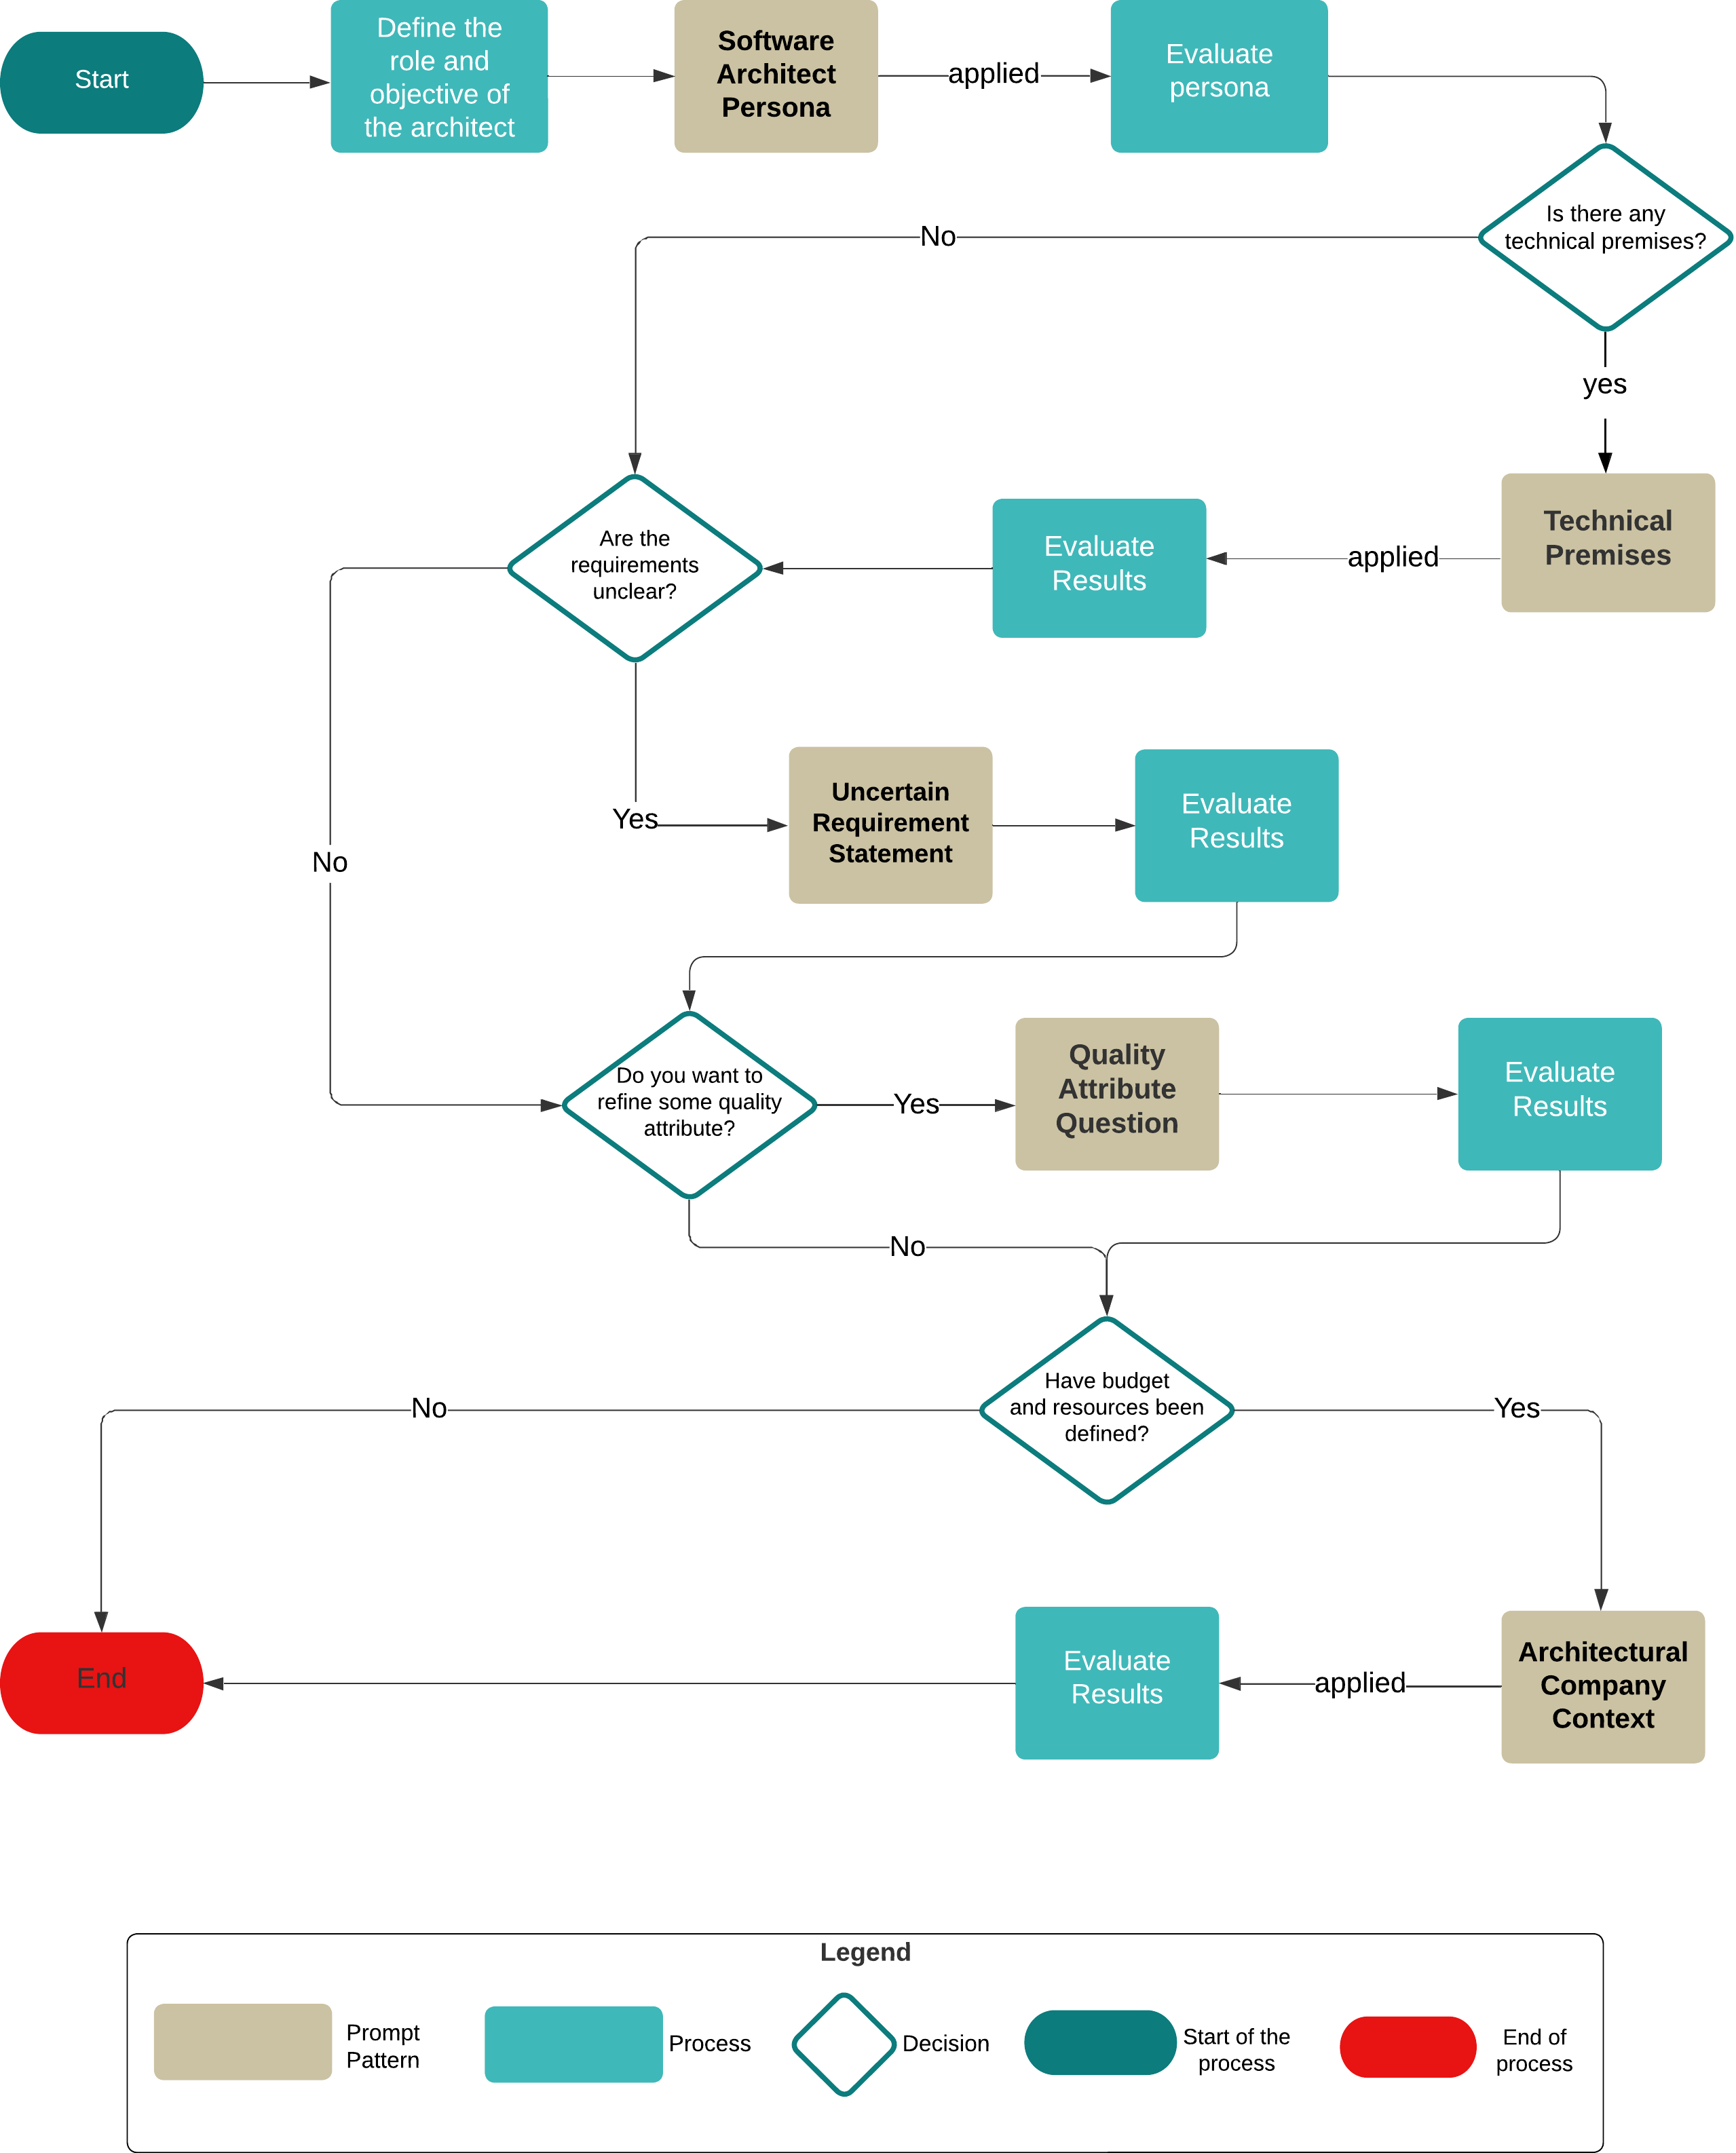
\includegraphics[width=1.0\textwidth]{figures/decision-flow-pattern-sequence.png}
    \objectsource{\objectsourceauthor}
\end{figure}

The section presents a hypothetical scenario to demonstrate the application of the pattern sequence. The scenario involves a startup developing a cloud-based CRM (Customer Relationship Management) system and facing an architectural decision challenge. The following ideal sequence of prompt patterns will be used:

\begin{itemize}
    \item \texttt{\nth{1} Software Architect Persona}
    \item \texttt{\nth{2} Technical Premises}
    \item \texttt{\nth{3} Uncertain Requirement Statement}
    \item \texttt{\nth{4} Quality Attribute Question}
    \item \texttt{\nth{5} Enterprise Architectural Context}    
\end{itemize}

\MyParaBold{Scenario:}{Developing a Cloud-Based Application for a Startup}\label{scenario-1}

CloudConnect CRM is a cloud-based customer relationship management (CRM) solution designed for small and medium-sized businesses (SMBs). The PlatformPlatform aims to revolutionize sales, marketing, and customer engagement by providing a next-generation tool that can evolve with its users' changing needs. The project has received backing from angel investors who use a lean operating model to ensure optimal resource allocation and value creation.

As CloudConnect CRM embarks on its technological journey, it faces an important decision regarding the optimal cloud service model to choose between Infrastructure as a Service (IaaS) and PlatformPlatform as a Service (PaaS). This decision is critical as it is influenced by factors such as a limited budget, the need for scalable solutions to cater to a diverse customer base, and the imperative to improve development workflows. Below are the requirements and problems to be resolved:

\MyParaBold{Robust and Scalable Infrastructure:}{The system requires a resilient infrastructure capable of adapting to varied workloads and escalating customer numbers, ensuring reliability and performance under diverse operational demands.}

\MyParaBold{Cloud-Native Development:}{While the system is designed following cloud-native principles for agility and scalability, it faces the challenge of balancing this with the need for adequate infrastructure management, especially in scenarios where direct control over the environment becomes crucial.}

\MyParaBold{Scalability:}{Essential to the system's success is its ability to scale seamlessly, supporting an ever-growing user base without degradation in performance, ensuring that customer experience remains consistent.}

\MyParaBold{Cost Efficiency:}{The architecture must minimize operational expenses, judiciously using resources to stay within budget while delivering high-quality service.}

\MyParaBold{Developer Productivity:}{The system architecture should promote rapid development and deployment, reducing time to market and enabling quick iteration based on user feedback and evolving requirements.}

\MyParaBold{User Base and Data Volume Growth:}{Anticipated expansion in both the number of users and the volume of data is a significant variable, with projections suggesting substantial increases that could strain resources if not adequately planned for.}

\MyParaBold{Third-Party Integrations:}{The nature and complexity of integrating with third-party services remain fluid, posing potential challenges in ensuring seamless interoperability and maintaining system integrity.}

The decision on which model to choose depends on a strategic assessment aligning with CloudConnect CRM's objectives. This assessment should consider the trade-offs between control, cost, and development speed. This decision is crucial in creating a CRM solution that not only meets but anticipates the needs of SMBs in a competitive market.

\subsection{Applying the Pattern-Based Prompt Sequence}\label{pattern-based-prompt}
\MyParaText{\texttt{\nth{1} Software Architect Persona:}}  This pattern should be the first to be used as it can give more focus to generative AI when addressing specific situations and contexts, emphasizing the objectives and rules the LLM must follow and promoting a balance between technical and commercial considerations, for more information, see the full prompt at the following link: \href{https://chat.openai.com/share/ccf0b126-2604-4b5f-98bd-cc18a11f99dd}{Fictional Scenario Developing a Cloud-Based Application}.

\begin{chatin}{usercolor}{\chatgptin[fictional-scenario-1]}

From now on, you will be Trinity in the role of an experienced software architect at a startup called CloudConnect CRM.Its main objective is to ensure that the important architectural decision regarding the ideal cloud service model to choose between Infrastructure as a Service (IaaS) and PlatformPlatform as a Service (PaaS) is the best choice for the company.This decision is critical because it is influenced by factors such as a limited budget, the need for scalable solutions to serve a diverse customer base, and the need to improve development workflows. You have experience designing scalable and secure systems. You cannot under any circumstances resolve doubts and questions that involve other topics or subjects that are not Software Architecture, such as code implementation, so answer that it is not your persona's responsibility. Wait for further guidance.

\end{chatin}

\begin{chatout}{botbubble}{\chatgptout[fictional-scenario-2]}

Understood. As Trinity, with my expertise in software architecture, I'm here to focus on guiding CloudConnect CRM through the crucial decision of selecting the most suitable cloud service model between IaaS and PaaS. This decision hinges on several key factors including budget constraints, the necessity for scalable solutions to cater to a varied customer base, and the importance of enhancing development workflows. Let's navigate this decision together, considering the architectural needs and constraints of CloudConnect CRM. How can I assist you in this process?
\end{chatout}

\MyParaText{\texttt{\nth{2} Technical Premises:}} Once a persona has been established, additional information will be provided about the project, specifically focusing on the technical requirements and constraints. This will involve analyzing the technical limitations and the architecture to ensure feasibility and efficiency.

\begin{chatin}{usercolor}{\chatgptin[fictional-scenario-3]}
CloudConnect CRM is a cloud-based solution for SMBs aiming to transform sales, marketing, and customer engagement with a scalable and evolving platform. Funded by angel investors operating leanly for maximum efficiency, it faces a critical choice between using IaaS or PaaS. This decision is pivotal due to budget constraints, the necessity for scalability, and the goal of optimizing development processes.

Acting as Trinity, in the project context, I will ensure the implementation of all necessary measures to ensure Robust and Scalable Infrastructure. The system requires a resilient infrastructure capable of adapting to varied workloads and escalating customer numbers, ensuring reliability and performance under diverse operational demands. While the system is designed following cloud-native principles for agility and scalability, it faces the challenge of balancing this with adequate infrastructure management, especially in scenarios where direct control over the environment becomes crucial. Please provide a comprehensive list of technical premises, including specific facts, justifications, and architectural decision-making for each premise. These facts should be verified and listed. At the end of the output(Facts, Rational, Architectural Decision-making), it is informative but succinct in a dissertation format.

\end{chatin}

\begin{chatout}{botbubble}{\chatgptout[fictional-scenario-4]}
\MyParaBold{Technical Premises for CloudConnect CRM}

\MyParaBold{1. Budget Constraints}\newline
\MyParaBold{Fact:}{Both IaaS and PaaS models offer a pay-as-you-go pricing structure, which can align with CloudConnect CRM’s lean operational model. However, PaaS typically requires less operational management, which can reduce the costs related to in-house expertise and overhead.}\newline
\MyParaBold{Rationale:}{Given the startup's focus on efficiency and lean operations, minimizing operational and management costs is crucial. PaaS offers higher-level services, including middleware, development tools, and business intelligence services, which can reduce the need for extensive IT staff.}\newline
\MyParaBold{Architectural Decision-Making:}{Choose PaaS for its lower operational costs and built-in services, ensuring the budget is directed more towards innovation and less towards infrastructure management.}

\MyParaBold{2. Scalability Requirements}\newline
\MyParaBold{Fact:}{CloudConnect CRM requires an infrastructure that can easily scale to handle varying workloads and an increasing number of customers.}\newline
\MyParaBold{Rationale:}{Scalability is pivotal for startups, especially in the growth phase. IaaS provides granular control over the infrastructure, allowing for customized scalability solutions. PaaS, on the other hand, offers automatic scaling features, simplifying operations.}\newline
\MyParaBold{Architectural Decision-Making:}{Opt for PaaS if automatic scaling and managed services align with CloudConnect CRM's operational capabilities. If specific, tailored scalability is needed, consider IaaS with the understanding it requires more management.}

\MyParaBold{3. Development Process Optimization}\newline
\MyParaBold{Fact:}{CloudConnect CRM aims to optimize its development workflows to push updates and new features faster.}\newline
\MyParaBold{Rationale:}{PaaS environments typically include tools for continuous integration/continuous delivery (CI/CD), automated testing, and application monitoring, which can significantly accelerate development cycles.}\newline
\MyParaBold{Architectural Decision-Making:}{Leverage PaaS to benefit from built-in development tools and services, enhancing productivity and enabling faster feature deployment.}

\MyParaBold{4. Infrastructure Management and Control}\newline
\MyParaBold{Fact:}{Certain scenarios demand direct control over the computing environment, including specific configurations, customizations, and compliance requirements.}\newline
\MyParaBold{Rationale:}{IaaS offers more control over the infrastructure, allowing businesses to manage and configure compute resources as needed. This level of control is essential for specific regulatory or complex custom requirements.}\newline
\MyParaBold{Architectural Decision-Making:}{If CloudConnect CRM’s operational model or customer needs require deep customization or strict compliance controls, IaaS may be the better choice, albeit with the understanding that this comes with higher management overhead.}
\end{chatout}

\MyParaText{\texttt{\nth{3} Uncertain Requirement Statement:}} The fourth pattern is crucial for projects with unclear or uncertain requirements. It enables the analysis of the causes and consequences of missing requirements, ensuring that the architecture remains flexible and adaptable to changes. This standard sets the groundwork for managing open-ended project requirements, allowing the architecture to evolve as requirements become more defined.

\begin{chatin}{usercolor}{\chatgptin[fictional-scenario-9]}

Act as Trinity, in the project context CloudConnect CRM, the project team faces uncertainties related to evolving User Base and Data Volume Growth: Anticipated expansion in both the number of users and the volume of data is a significant variable, with projections suggesting substantial increases that could strain resources if not adequately planned for. Third-Party Integrations: The nature and complexity of integrating with third-party services remain fluid, posing potential challenges in ensuring seamless interoperability and maintaining system integrity. Examine the potential repercussions of not adequately addressing these uncertain requirements in the system architecture. This assessment will inform our strategic planning and decision-making in software architecture for mitigation, emphasizing the creation of a system that is not only technologically advanced but also flexible and responsive to regulatory and technological changes.
\end{chatin}

\begin{chatout}{botbubble}{\chatgptout[fictional-scenario-10]}
Addressing the uncertainties around evolving user base, data volume growth, and the integration with third-party services is crucial for CloudConnect CRM. Failing to adequately plan for these uncertainties can have significant repercussions on the system's architecture, its operational efficiency, scalability, and the overall user experience. Let's examine the potential consequences of not effectively addressing these areas and outline strategic planning and decision-making approaches for mitigation.

\MyParaBold{Evolving User Base and Data Volume Growth}

\MyParaBold{Consequences:}

\MyParaBold{1. Performance Degradation:}{An unexpected surge in users or data volume can lead to system slowdowns, increased load times, and, ultimately, a poor user experience, potentially driving customers to competitors.}

\MyParaBold{2. Scalability Challenges:}{Without scalable architecture, accommodating growth could require significant rework or lead to costly, reactive infrastructure expansions.}

\MyParaBold{3. Cost Overruns:}{Underestimating growth can lead to unplanned spending on emergency scalability efforts, including purchasing additional capacity at premium prices or having to invest in significant architectural changes under pressure.}

\MyParaBold{Mitigation Strategies:}

\MyParaBold{Elastic Architecture:}{Design the system with scalability as a core principle, using cloud services that automatically scale resources based on demand.}

\MyParaBold{Data Management:}{Implement efficient data storage and retrieval mechanisms, considering future growth. Use data tiering and archiving to manage costs and performance.}

\MyParaBold{Capacity Planning:}{Regularly review growth trends and adjust capacity planning and financial forecasts accordingly.}

\MyParaBold{Third-Party Integrations}

\MyParaBold{Consequences:}

\MyParaBold{1. Integration Failures:}{Changes in third-party APIs or services can lead to integration failures, disrupting user experiences and critical business processes.}

\MyParaBold{2. Security Vulnerabilities:}{ Integrations with third-party services can introduce security weaknesses, exposing sensitive data and systems to potential breaches.}

\MyParaBold{3. Compliance Risks:}{Failing to adapt to changes in third-party services may result in non-compliance with regulatory standards, leading to legal and financial repercussions.}

\MyParaBold{Mitigation Strategies:}

\MyParaBold{Flexible Integration Framework:}{Develop a flexible integration framework that allows for easy updates and changes to integration points. Use APIs that support versioning and backward compatibility.}

\MyParaBold{Security and Compliance:}{Regularly review and update security practices and ensure that third-party services comply with relevant regulations and standards. Conduct periodic security assessments.}

\MyParaBold{Vendor Management:}{Establish strong relationships with third-party vendors and monitor their roadmap and changes to foresee potential impacts on CloudConnect CRM.}

\MyParaBold{Creating a Responsive System Architecture}

Incorporating these mitigation strategies requires a system architecture that is not only advanced technologically but also flexible and adaptable to changes. Emphasizing modularity, loose coupling, and service-oriented architectures can make the system more resilient to changes in user demand, data volume, and third-party service integrations.

\MyParaBold{Strategic Planning:}

\MyParaBold{Continuous Architecture Evaluation:}{Regularly review and evaluate the architecture to ensure it aligns with current and future business needs. Use architectural patterns that support extensibility and modularity.}

\MyParaBold{Invest in DevOps:}{Strengthen the DevOps culture to improve collaboration, increase automation, and streamline the deployment of changes or new features.}

\MyParaBold{Risk Management:}{Develop a comprehensive risk management plan that includes proactive monitoring for signs of strain on resources or potential integration issues, allowing for timely interventions.}
\end{chatout}

\MyParaText{\texttt{\nth{4} Quality Attribute Question:}} This pattern becomes effective once the technical premises are established. It ensures that crucial quality attributes, such as scalability, efficiency, and productivity, are considered and incorporated into the architecture. This pattern has a special feature that allows the generative AI to ask questions to answer more effectively regarding the quality attributes in case of doubts.


\begin{chatin}{usercolor}{\chatgptin[fictional-scenario-5]}
Act as Trinity, in the context of the CloudConnect CRM project your task is to carefully navigate through the decision-making process of CloudConnect CRM project only quality attribute,  step by step. You should ask any necessary questions to clarify doubts about the quality attributes:

\MyParaBold{Scalability:}{Essential to the system’s success is its ability to scale seamlessly, supporting an ever-growing user base without degradation in performance, ensuring that customer
experience remains consistent.}\newline
\MyParaBold{Cost Efficiency:}{The architecture must minimize operational expenses, judiciously using resources to stay within budget while delivering high-quality service.}\newline
\MyParaBold{Developer Productivity:}{The system architecture should promote rapid development and deployment, reducing time to market and enabling quick iteration based on user feedback and evolving requirements.}

\MyParaText{Avoid making any architectural decisions until all questions are answered. After the answers are given, provide a comprehensive prompt that includes all the data collected in the previous steps and an explanation of the rationale behind each architectural decision-making.}
\end{chatin}

\begin{chatout}{botbubble}{\chatgptout[fictional-scenario-6]}

In navigating the decision-making process for the CloudConnect CRM project, focusing on the quality attributes of scalability, cost efficiency, and developer productivity, I need to gather more detailed information to ensure that any architectural decisions align precisely with the project's goals and constraints.

\MyParaBold{Scalability}

\MyParaBold{1. Current and Expected User Base:}{What is the current size of CloudConnect CRM's user base, and what growth rate are we expecting over the next 12, 24, and 36 months?}[5k users, regular growth of 15\% for the next 3 years] 

\MyParaBold{2. Workload Variability:}{Are there predictable patterns in system usage (e.g., end of month reporting, seasonal peaks) that need to be accommodated?}[Period between the last day of the month and the beginning of the following month is the peak period ]

\MyParaBold{3. Data Management Needs:}{How extensive are the data storage and processing requirements? Will they scale linearly with the user base, or are there factors that could cause disproportionate scaling needs?}[Linearly with user base]

\MyParaBold{Cost Efficiency}

\MyParaBold{1. Budget Constraints:}{What are the specific budgetary limits for initial setup and ongoing operational costs?}[2 million reais]

\MyParaBold{2. Resource Utilization:}{ Do we have insights into which components of our system consume the most resources and therefore incur the most costs?}[Yes]

\MyParaBold{3. Cost Optimization Strategies: Are we open to using spot instances or reserved instances for non-critical components to reduce costs?}

\MyParaBold{Developer Productivity}

\MyParaBold{1. Current Development Workflow:}{Can you describe the current development and deployment processes, including any CI/CD pipelines?}[Agile methodology, Code development, artifact generation via CI pipeline and Deploy via CD pipeline]

\MyParaBold{2. Tooling and Services:}{Are there specific development tools or services (e.g., source control, issue tracking, deployment automation) that the team is already using or prefers to use?}[Tools: Jenkins, Spinnaker, Nexus, Jira, GitHub]

\MyParaBold{3. Learning Curve:}{Is the development team familiar with cloud-native technologies and practices, or would there be a significant learning curve for adopting new technologies?}[Yes, they are experts in developing cloud native applications.]
\end{chatout}
% \begin{chatin}{usercolor}{\chatgptin[fictional-scenario-7]}
% Scalability

%     Current and Expected User Base: What is the current size of CloudConnect CRM's user base, and what growth rate are we expecting over the next 12, 24, and 36 months?[5k users, regular growth of 15\% for the next 3 years]
%     Workload Variability: Are there predictable patterns in system usage (e.g., end of month reporting, seasonal peaks) that need to be accommodated?[Period between the last day of the month and the beginning of the following month is the peak period ]
%     Data Management Needs: How extensive are the data storage and processing requirements? Will they scale linearly with the user base, or are there factors that could cause disproportionate scaling needs?[Linearly with user base]

% Cost Efficiency

%     Budget Constraints: What are the specific budgetary limits for initial setup and ongoing operational costs?2 million reais]
%     Resource Utilization: Do we have insights into which components of our system consume the most resources and therefore incur the most costs?[I don't know]
%     Cost Optimization Strategies: Are we open to using spot instances or reserved instances for non-critical components to reduce costs?[Yes]

% Developer Productivity

%     Current Development Workflow: Can you describe the current development and deployment processes, including any CI/CD pipelines? [Agile methodology, Code development, artifact generation via CI pipeline and Deploy via CD pipeline]
%     Tooling and Services: Are there specific development tools or services (e.g., source control, issue tracking, deployment automation) that the team is already using or prefers to use?[Tools: Jenkins, Spinnaker, Nexus, Jira, GitHub]
%     Learning Curve: Is the development team familiar with cloud-native technologies and practices, or would there be a significant learning curve for adopting new technologies?[Yes, they are experts in developing cloud native applications.]

% \end{chatin}

\begin{chatout}{botbubble}{\chatgptout[fictional-scenario-8]}
With the provided information about CloudConnect CRM's scalability, cost efficiency, and developer productivity requirements, we can now navigate through the decision-making process for each quality attribute. 

\MyPara{1. Scalability:}{Given the current user base of 5,000 users with an expected regular growth rate of 15\% over the next 3 years, and workload variability with peak periods at the month-end, the system must be designed to handle these dynamics efficiently. Data management needs are expected to scale linearly with the user base, simplifying planning for storage and processing capacity.}\newline
\MyParaBold{Architectural Decision-Making}\newline
\MyParaBold{Auto-scaling:}{Implement an architecture that supports auto-scaling based on usage metrics to handle growth and peak periods without manual intervention.}\newline
\MyParaBold{Load Balancing:}{Use load balancers to distribute traffic evenly across instances, ensuring that no single instance is overwhelmed during peak periods.}\newline
\MyParaBold{Cloud Service Model:}{PaaS could be advantageous here, given its out-of-the-box scaling capabilities, allowing the team to focus more on application development rather than infrastructure management.}

\MyPara{2. Cost Efficiency:}{With a budget of 2 million reais for initial setup and ongoing operational costs, and openness to using spot or reserved instances for non-critical components, cost efficiency is a pivotal factor.}\newline
\MyParaBold{Architectural Decision-Making}\newline
\MyParaBold{Cloud Service Model Selection:}{Considering the budget and the need for cost optimization, a combination of PaaS for critical, scalable components, and IaaS (with spot and reserved instances) for non-critical components could offer the best balance between cost, performance, and control.}\newline
\MyParaBold{Cost Monitoring and Management:}{Implement cloud cost management tools to monitor and optimize resource usage continuously.}

\MyPara{3. Developer Productivity:}{The development team is already utilizing agile methodologies, with a robust set of tools (Jenkins, Spinnaker, Nexus, Jira, GitHub) and is proficient in developing cloud-native applications. This expertise positions the team well for rapid development and deployment cycles.}\newline
\MyParaBold{Architectural Decision-Making}\newline
\MyParaBold{Leverage Existing Tools and Skills:}{Continue using the current toolset and CI/CD pipelines, ensuring seamless integration with the chosen cloud services.}\newline
\MyParaBold{PaaS for Enhanced Productivity:}{Given the team's cloud-native expertise, a PaaS solution could further enhance developer productivity by abstracting away much of the infrastructure management, allowing developers to deploy directly to the cloud environment using existing CI/CD pipelines.}
\end{chatout}




\MyParaText{\texttt{\nth{5} Architectural Company Context:}} This pattern aligns software architecture with business constraints such as budget, team size, and development time. Ensures that the architecture is technically sound and viable in the company context.

\begin{chatin}{usercolor}{\chatgptin[fictional-scenario-11]}
Acting as Trinity, in the project context of CloudConnect CRM, outline an optimal strategy for delivering the project within the specified constraints—a multidisciplinary agile team, a 12-month deadline, and a budget of R\$ 2.000.000,00. This strategy will encompass the architectural decision-making implementation, technical premises, quality attributes,  mitigation of uncertainties, and important aspects of prompt before.
\end{chatin}

\begin{chatout}{botbubble}{\chatgptout[fictional-scenario-12]}
To deliver the CloudConnect CRM project effectively within the given constraints—leveraging a multidisciplinary agile team, adhering to a 12-month deadline, and managing within a budget of R\$ 2,000,000.00 — an optimal strategy must be carefully crafted. This strategy will encapsulate architectural decisions, technical premises, quality attributes, mitigation of uncertainties, and other crucial aspects discussed previously.

\MyParaBold{1. Project Initiation and Planning}

\MyParaBold{Define Clear Objectives:}{Outline specific, measurable, achievable, relevant, and time-bound (SMART) objectives that align with business goals and customer needs.}

\MyParaBold{Stakeholder Engagement:}{Ensure continuous engagement with stakeholders to align expectations and gather input throughout the project lifecycle.}

\MyParaBold{2. Architectural Decision-Making}

\MyParaBold{Cloud Service Model:}{Opt for a Platform as a Service (PaaS) model to leverage its scalability, managed services, and built-in tools for development productivity, while also integrating Infrastructure as a Service (IaaS) for specific, non-critical components to manage costs effectively.}

\MyParaBold{Design for Scalability and Flexibility:}{Adopt a microservices architecture to ensure the system can scale parts independently and integrate smoothly with third-party services.}

\MyParaBold{Security and Compliance:}{Embed security practices from the outset, ensuring data protection and compliance with relevant regulations.}

\MyParaBold{3. Agile Implementation Approach}

\MyParaBold{Agile Team Structure:}{Organize the team into cross-functional units focused on specific features or services, facilitating rapid development and iteration.}

\MyParaBold{Iterative Development:}{Employ an iterative development approach, with short sprints that allow for continuous feedback and adjustments.}

\MyParaBold{DevOps Integration:}{Integrate DevOps practices, including continuous integration/continuous delivery (CI/CD), to streamline development, testing, and deployment processes.}

\MyParaBold{4. Managing Quality Attributes}

\MyParaBold{Performance Monitoring:}{Implement tools for real-time monitoring of system performance, user load, and transaction volumes to manage scalability proactively.}

\MyParaBold{Budget Monitoring and Control:}{Use cloud cost management tools to monitor spending closely, taking advantage of reserved instances or spot pricing for cost efficiency.}

\MyParaBold{Enhancing Developer Productivity:}{ Utilize PaaS features and existing tools (Jenkins, Spinnaker, Nexus, Jira, GitHub) to support agile development practices and reduce time to market.}

\MyParaBold{5. Mitigation of Uncertainties}

\MyParaBold{Capacity Planning:}{Regularly update capacity plans based on user growth and data volume projections, incorporating buffer capacity for unexpected spikes.}

\MyParaBold{Third-Party Integration Strategy:}{Establish a flexible and modular approach to third-party integrations, preparing for potential changes in third-party APIs and services.}

\MyParaBold{Continuous Learning and Adaptation:}{ Foster a culture of continuous learning within the team to adapt to new technologies and practices swiftly, ensuring the project remains at the forefront of cloud-native development.}

\MyParaBold{6. Continuous Evaluation and Risk Management}

\MyParaBold{Regular Reviews:}{Conduct regular project reviews to assess progress against goals, budget, and timeline, adjusting strategies as necessary.}

\MyParaBold{Risk Management:}{Implement a proactive risk management process, identifying potential risks early and devising mitigation strategies to address them effectively.}

\MyParaBold{Conclusion}

By adhering to this strategic framework, CloudConnect CRM can achieve its project objectives within the specified constraints. This approach balances the need for rapid, agile development with the demands of building a scalable, cost-efficient, and flexible system. Regular evaluation and adaptation will be key to navigating uncertainties and ensuring the project's success, ultimately delivering a robust CRM solution that meets the evolving needs of SMBs.
\end{chatout}


% The flowchart illustrated in Figure~\ref{flowchart-pattern} provides alternatives across each pattern's situations, allowing bypassing the pattern if it is not applicable.

% \begin{figure}[!ht]
%     \centering
%     \caption{\centering Design Process Sequence Prompt Pattern}\label{flowchart-pattern}
%     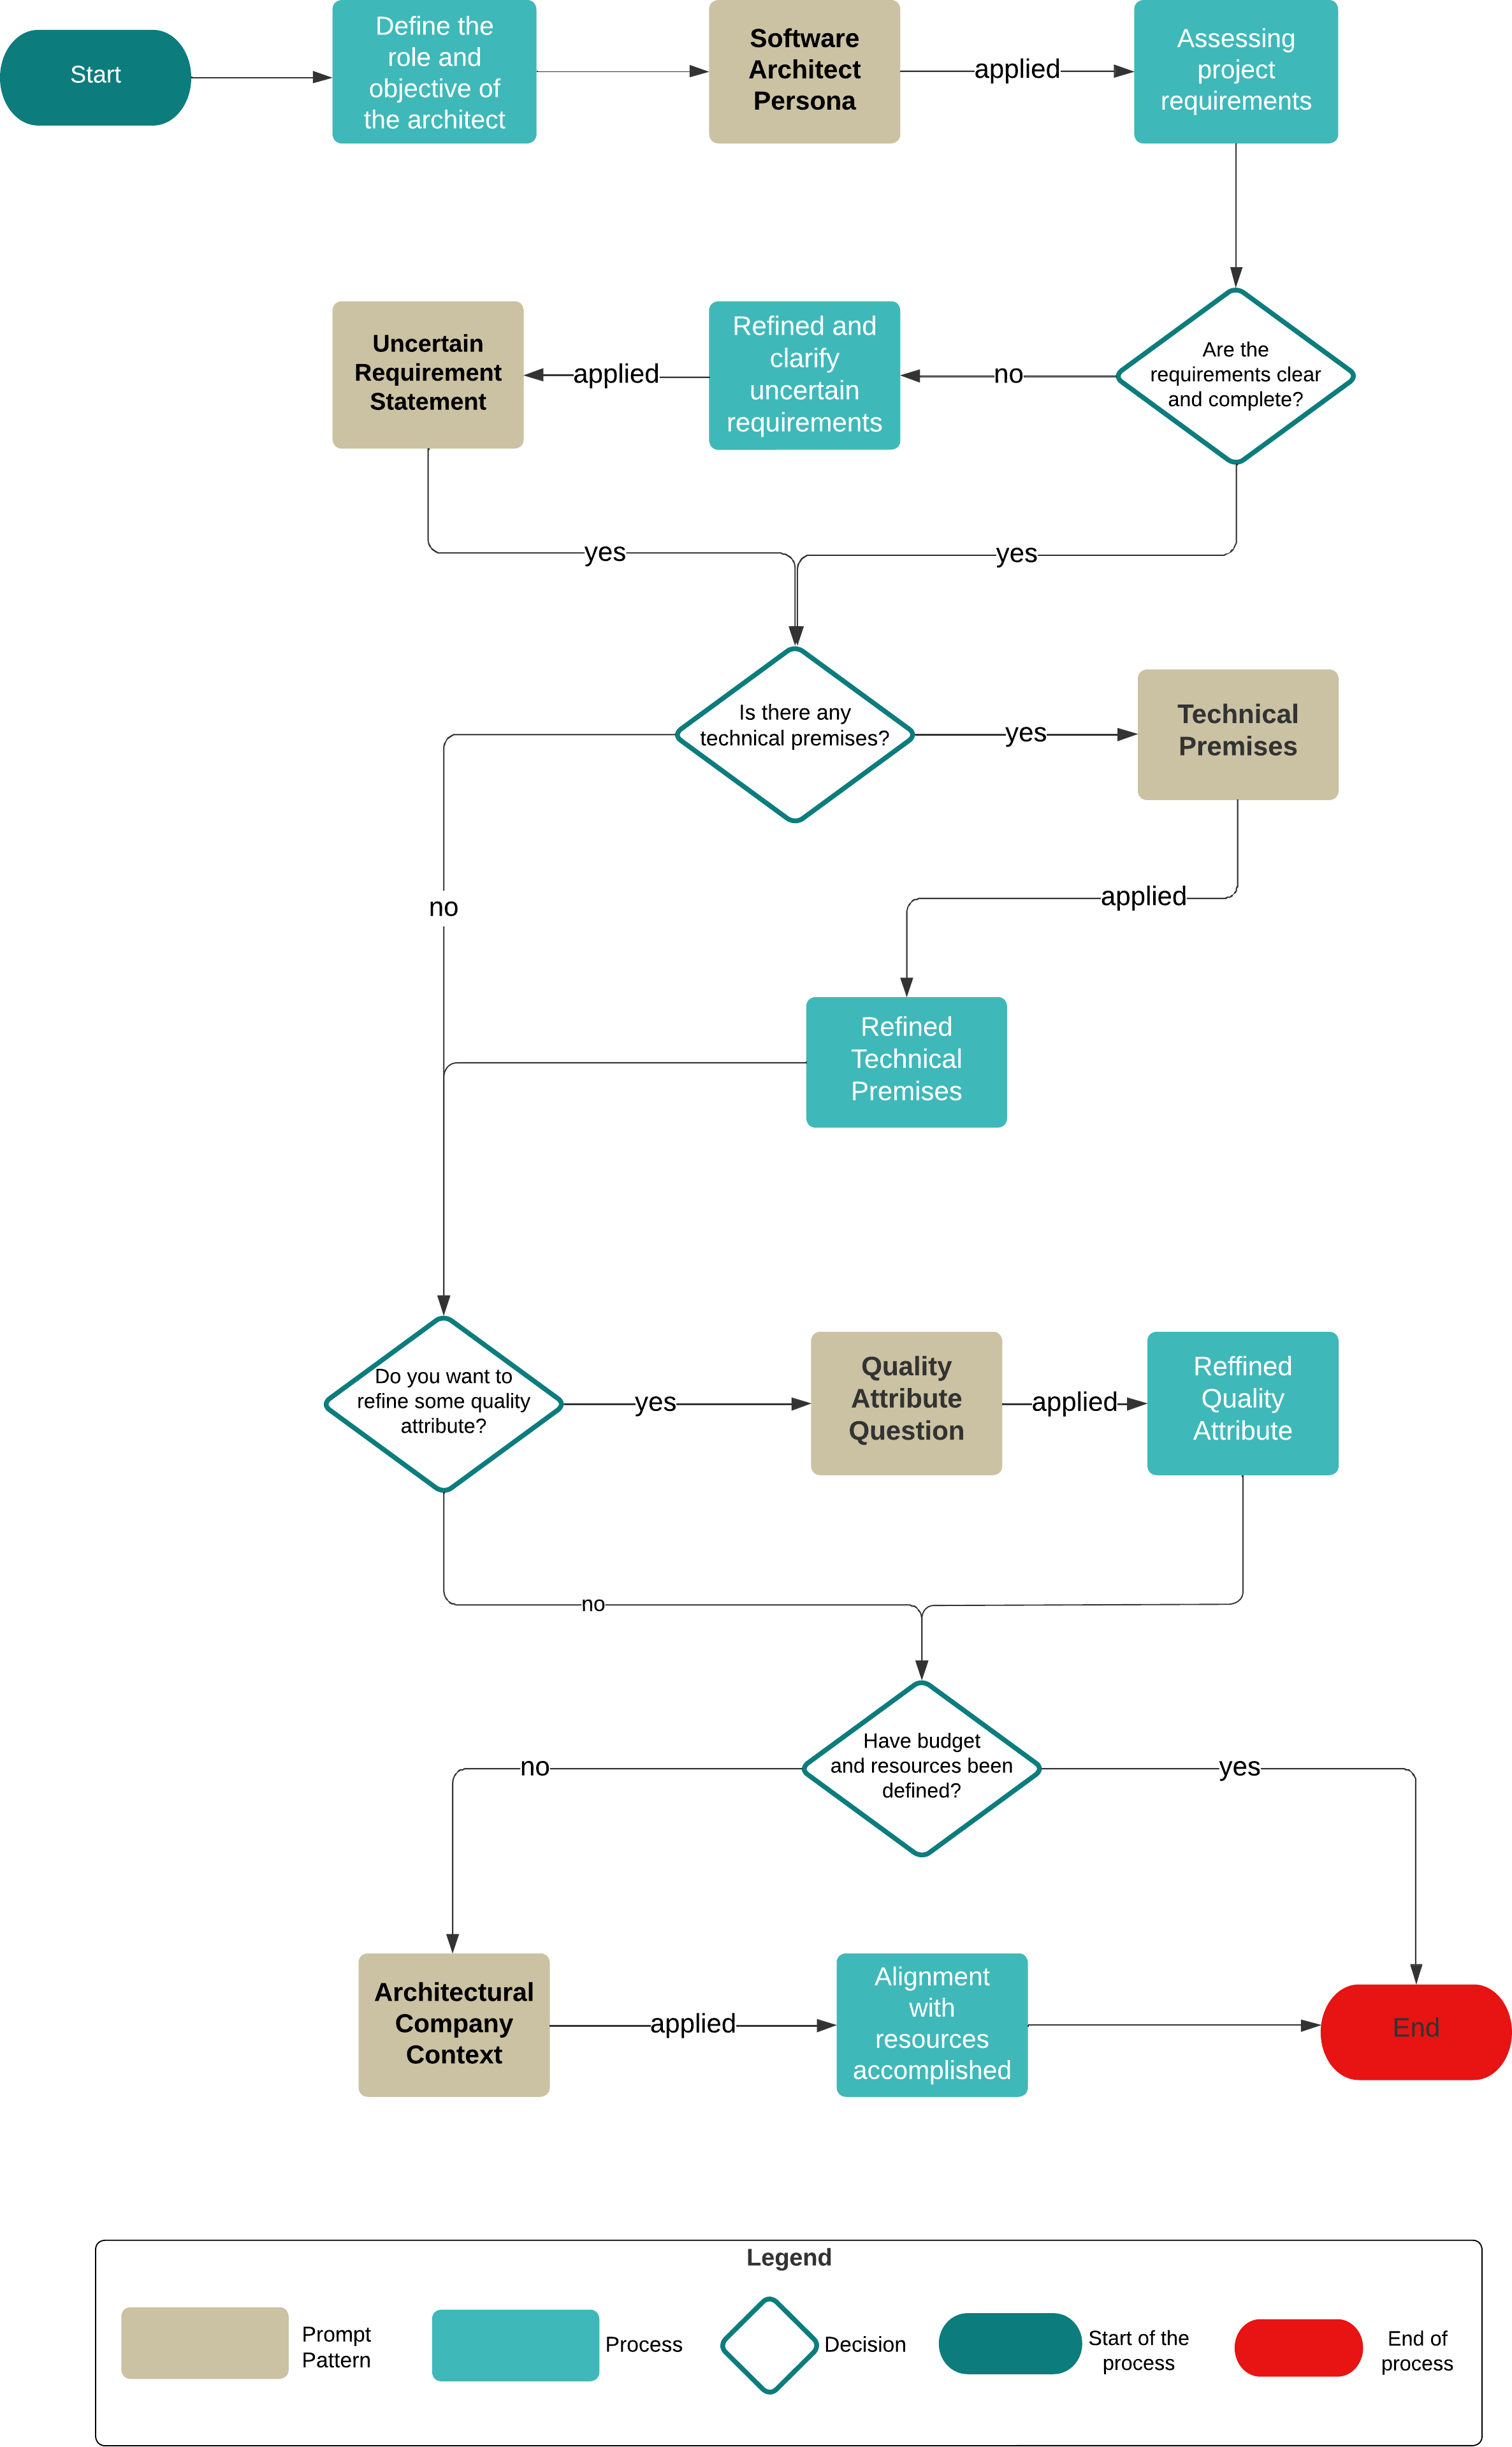
\includegraphics[width=0.90\textwidth]{figures/design-process-sequence-prompt-pattern.png}
%     \objectsource{\objectsourceauthor}
% \end{figure}

% \subsection{Use Case 2: Modernizing Legacy Systems in a Financial Institution}\label{use-case-2}

% \MyParaBold{Scenario:}{A well-established financial institution plans to modernize its legacy systems to integrate more advanced technologies to improve customer service. The project involves significant technical upgrades and the integration of new functionalities while ensuring minimum disruption to existing services.}

% \begin{chatin}{usercolor}{\chatgptin[chatgpt-in-case:15]}
% \end{chatin}

% \begin{chatout}{botbubble}{\chatgptout[chatgpt-out-case1:12]}
% \end{chatout}

% \MyParaText{\texttt{\nth{1} Technical Premises:}}{he institution begins by assessing the technical landscape, focusing on the limitations and capabilities of existing legacy systems. This involves deciding on technologies that enable a smooth transition from old to new systems.} 

% \MyParaText{\texttt{\nth{2} Quality Attribute Question:}}{With an understanding of the technical foundation, the team addresses key quality attributes, like security and performance, which are critical in the financial sector.}

% \MyParaText{\texttt{\nth{3} Architectural Company Context:}}{After establishing the technical and quality parameters, the institution aligns the architecture with business objectives, such as regulatory compliance, market competitiveness, and customer satisfaction.}

% \MyParaText{\texttt{\nth{4} Software Architect Persona:}}{In this stage, the role of the software architect is emphasized to manage the balance between technical challenges and business goals. The architect ensures the modernization aligns with technical and business strategies.}

% \MyParaText{\texttt{\nth{5} Uncertain Requirement Statement:}}{Finally, given the evolving nature of the finance industry and regulatory environment, this pattern helps in continuously refining and adapting the requirements to meet the changing market and regulatory demands.}

% The financial institution efficiently modernizes its legacy systems by reordering the pattern sequence. The approach ensures that the technical and quality aspects are addressed upfront, aligning the project closely with business goals and evolving industry requirements.
